\documentclass[a4paper, 11pt]{report}
\usepackage{blindtext}
\usepackage[T1]{fontenc}
\usepackage[utf8]{inputenc}
\usepackage{titlesec}
\usepackage{fancyhdr}
\usepackage{geometry}
\usepackage{fix-cm}
\usepackage[hidelinks]{hyperref}
\usepackage{graphicx}
\usepackage{titlesec}

\usepackage[english]{babel}

\geometry{ margin=30mm }
\counterwithin{subsection}{section}
\renewcommand\thesection{\arabic{section}.}
\renewcommand\thesubsection{\thesection\arabic{subsection}.}
\usepackage{tocloft}
\renewcommand{\cftchapleader}{\cftdotfill{\cftdotsep}}
\renewcommand{\cftsecleader}{\cftdotfill{\cftdotsep}}
\setlength{\cftsecindent}{2.2em}
\setlength{\cftsubsecindent}{4.2em}
\setlength{\cftsecnumwidth}{2em}
\setlength{\cftsubsecnumwidth}{2.5em}

\titlespacing\section{0pt}{12pt plus 4pt minus 2pt}{0pt plus 2pt minus 2pt}
\titlespacing\subsection{0pt}{12pt plus 4pt minus 2pt}{0pt plus 2pt minus 2pt}

\begin{document}
\titleformat{\section}
{\normalfont\fontsize{15}{0}\bfseries}{\thesection}{1em}{}
\titlespacing{\section}{0cm}{0.5cm}{0.15cm}
\titleformat{\subsection}
{\normalfont\fontsize{13}{0}\bfseries}{\thesubsection}{0.5em}{}
\titlespacing{\section}{0cm}{0.5cm}{0.15cm}

%=============================================================================

\pagenumbering{Alph}
\begin{titlepage}
\begin{flushright}

\includegraphics[width=4cm]{USyd}\\[2cm]
\end{flushright}
\center 
\textbf{\huge INFO1111: Computing 1A Professionalism}\\[0.75cm]
\textbf{\huge 2023 Semester 1}\\[2cm]
\textbf{\huge Self-Learning Report}\\[3cm]

\textbf{\huge Submission number: 3}\\[0.75cm]
\textbf{Github link: https://github.com/Blackhistoryw/Info1111- }\\[2cm]

{\large
\begin{tabular}{|p{0.35\textwidth}|p{0.55\textwidth}|}
	\hline
	{\bf Student name} & Xinning Wu\\
	{\bf Student ID} & 500318346\\
	{\bf Topic} & Using JavaScript to make a online search website \textit{Note: This must be the same as was in your topic approval}\\
	{\bf Levels already achieved} & no\\
	{\bf Levels in this report} & A B C\\
	\hline
\end{tabular}
}
\thispagestyle{empty}
\end{titlepage}
\pagenumbering{arabic}


%=============================================================================

\tableofcontents

%=============================================================================


%=============================================================================


\newpage
\section{Level A: Initial Understanding}
\vspace{5mm}
\subsection{Level A Demonstration}
List the three things you will do to demonstrate your understanding of this topic.

To demonstrate my understanding of completing a video browsing website with JavaScript, I would take the following steps:
\begin{itemize}
\item Concept Explanation: First, I would describe the key concepts and components required in building a video browsing website. This would include elements like HTML and CSS for the website structure and style, JavaScript for interactivity, and APIs like the HTML5 Video API for handling video playback. I'd also discuss server-side concepts, including database design for storing video metadata, and how to handle user authentication if necessary.

\item Detailed Walkthrough of Implementation: Next, I would delve into the specifics of the implementation. I would start by explaining how to design the HTML structure of the web pages and apply styles using CSS. I would also talk about the use of JavaScript to add interactivity to the website, such as playing videos, pausing, fast-forwarding, and even implementing a video search function. This could involve using Ajax calls or Fetch API to retrieve video details from the server, or using the JavaScript built-in functions to control video playback.

\item Practical Demonstration: Finally, I would provide a practical, step-by-step demonstration or code example showcasing how to bring all these elements together to create a functional video browsing website. This would cover creating an HTML template for the video player and the video gallery, styling it with CSS, and adding the JavaScript code necessary to load and control the videos. I would also demonstrate how to handle server-side tasks, like retrieving video details from a database and sending them to the client side.
\end{itemize}
Each of these steps would aim to provide a comprehensive understanding of how to build a video browsing website using JavaScript, from the broad concepts to the specific implementation details.

\textit{Note: This must be the same as was in your topic approval}


\subsection{Learning Approach}
I first approached learning JavaScript by  starting  the  JavaScript  beginner  track  by Youtube, here I learnt a good foundational understanding of JavaScript and how to start programming in it. After watching a part of the online video, I would pause and write my understanding of the  point  explained.  Treehouse also had  quizzes  and programming exercises in which I answered multiple choice questions about what I learnt and programmed some simple JavaScript in their online coding environment.

\subsubsection{}section{Start with the Basics:}

The first step to learning JavaScript is understanding the basics of the language.
Resources:
\begin{itemize}
\item	"JavaScript for Cats": An introduction for new programmers.
\item	"Eloquent JavaScript": A book about JavaScript and programming.
Key Topics:
\item	Variables and Data Types.
\item	Operators (Arithmetic, Assignment, Comparison, Logical, Bitwise).
\item	Control Flow (If..Else, Switch, For, While, Do-While).
\item	Functions and Scope.
\item	Arrays and Objects.
\item	Errors and Exception Handling.
\end{itemize}

\subsubsection{Understanding the Document Object Model (DOM)}

The DOM is a programming interface for web documents. It represents the structure of a document and allows a way to manipulate its content and visual presentation.
Resources:
\begin{itemize}
\item	"DOM Enlightenment": Exploring the relationship between JavaScript and the modern HTML DOM.
\item	Mozilla Developer Network (MDN) DOM Documentation: Comprehensive documentation on the DOM.
Key Topics:
\item	Selecting Elements.
\item	Changing Elements.
\item	Adding and Deleting Elements.
\item	Document and Element properties.
\item	Event Handling.
\end{itemize}

\subsubsection{Dive into Advanced Concepts}

After grasping the basics, I try to learn the more complex aspects of JavaScript.
Resources:
\begin{itemize}
\item	"You Don’t Know JS": A book series which dives deep into the core mechanisms of JavaScript.
\item	"JavaScript: The Good Parts": This book covers the better parts of JavaScript.
Key Topics:
\item	Closures.
\item	Prototypes and Inheritance.
\item	Promises and Async/Await.
\item	ES6+ features like Arrow Functions, Template Literals, Destructuring Assignment, etc.
\item	AJAX (Asynchronous JavaScript and XML).
\end{itemize}

\subsubsection{Practice Skills}

Learning programming isn't just about understanding the concepts. I also need to apply what I've learned.
Resources:
\begin{itemize}
\item	Codecademy: Offers interactive coding exercises with instant feedback.
\item	LeetCode: Focus on solving algorithm problems.
\item	FreeCodeCamp: Offers a full curriculum including a JavaScript algorithm scripting section.
\end{itemize}

\subsubsection{Learn a JavaScript Framework}

I explore JavaScript frameworks which make it easier to build complex applications.
Choose between:
\begin{itemize}
\item	React: Maintained by Facebook, used for building user interfaces, especially for single page applications.
\item	Angular: Maintained by Google, a complete framework including a lot of features out of the box.
\item	Vue.js: Easier to grasp for beginners, lightweight, and versatile.
\end{itemize}

\subsubsection{Build Projects}

Building my own projects not only helps solidify my skills, but also gives me something to show to potential employers.
Possible Project Ideas:
\begin{itemize}
\item	A ToDo List Application.
\item	A Simple Calculator.
\item	A Weather Forecast App using an API.
\end{itemize}

\subsection{Challenges and Difficulties}
Something I found difficult when learning JavaScript was interacting with HTML and CSS elements, it was difficult to find right functions and syntax to do exactly what I wanted. I found that I had to broaden my understanding of HTML and CSS to fully understand	niche	JavaScript	code. Another element of  learning  JavaScript  I  found  difficult  was understanding how memory and data was stored in the program. I needed to have data saved in the program when switching from my one page to my another page. I tried many methods until I came across local storage and had further difficulties trying to understand the difference between local and session storage.

\subsection{Learning Sources}
Learning Source - What source did you use? (Note: Include source details such as links to websites, videos etc.).	Contribution to Learning - How did the source contribute to your learning (i.e. what did you use the source for)?

\begin{tabular}{|p{0.45\textwidth}|p{0.45\textwidth}|}
	\hline
	Learning Source - What source did you use? (Note: Include source details such as links to websites, videos etc.). & Contribution to Learning - How did the source contribute to your learning (i.e. what did you use the source for)?\\
	\hline
	W3schools timing events: \url{https://www.w3schools.com/js/js_timing.asp} & help me understand basics of javascript\\
	\hline
	Stack Overflow Forums: \url{https://stackoverflow.com/questions/tagged/javascript} & help me issuing some tag problems\\
	\hline
	Youtube: \url{https://www.youtube.com/watch?v=PkZNo7MFNFg&ab_channel=freeCodeCamp.org} & help me deal with some code issues\\
	\hline
	MDN web docs: \url{https://developer.mozilla.org/en-US/search?q=JavaScript} & help me have a better understading of javascript\\

	\hline
\end{tabular}

\subsection{Application artifacts}
I have made a simple web program with multiple pages. In the pages, the program accepts two user inputs and lookups. The program checks if the user input is valid, and if it is, the program will put the video and URL, and juxtapose the descriptions in a list. The most recent record is displayed at the top of the list. Finally, the user can clear the data with a button on the page. My project folder is attached to this submission.

\newpage

\begin{figure}
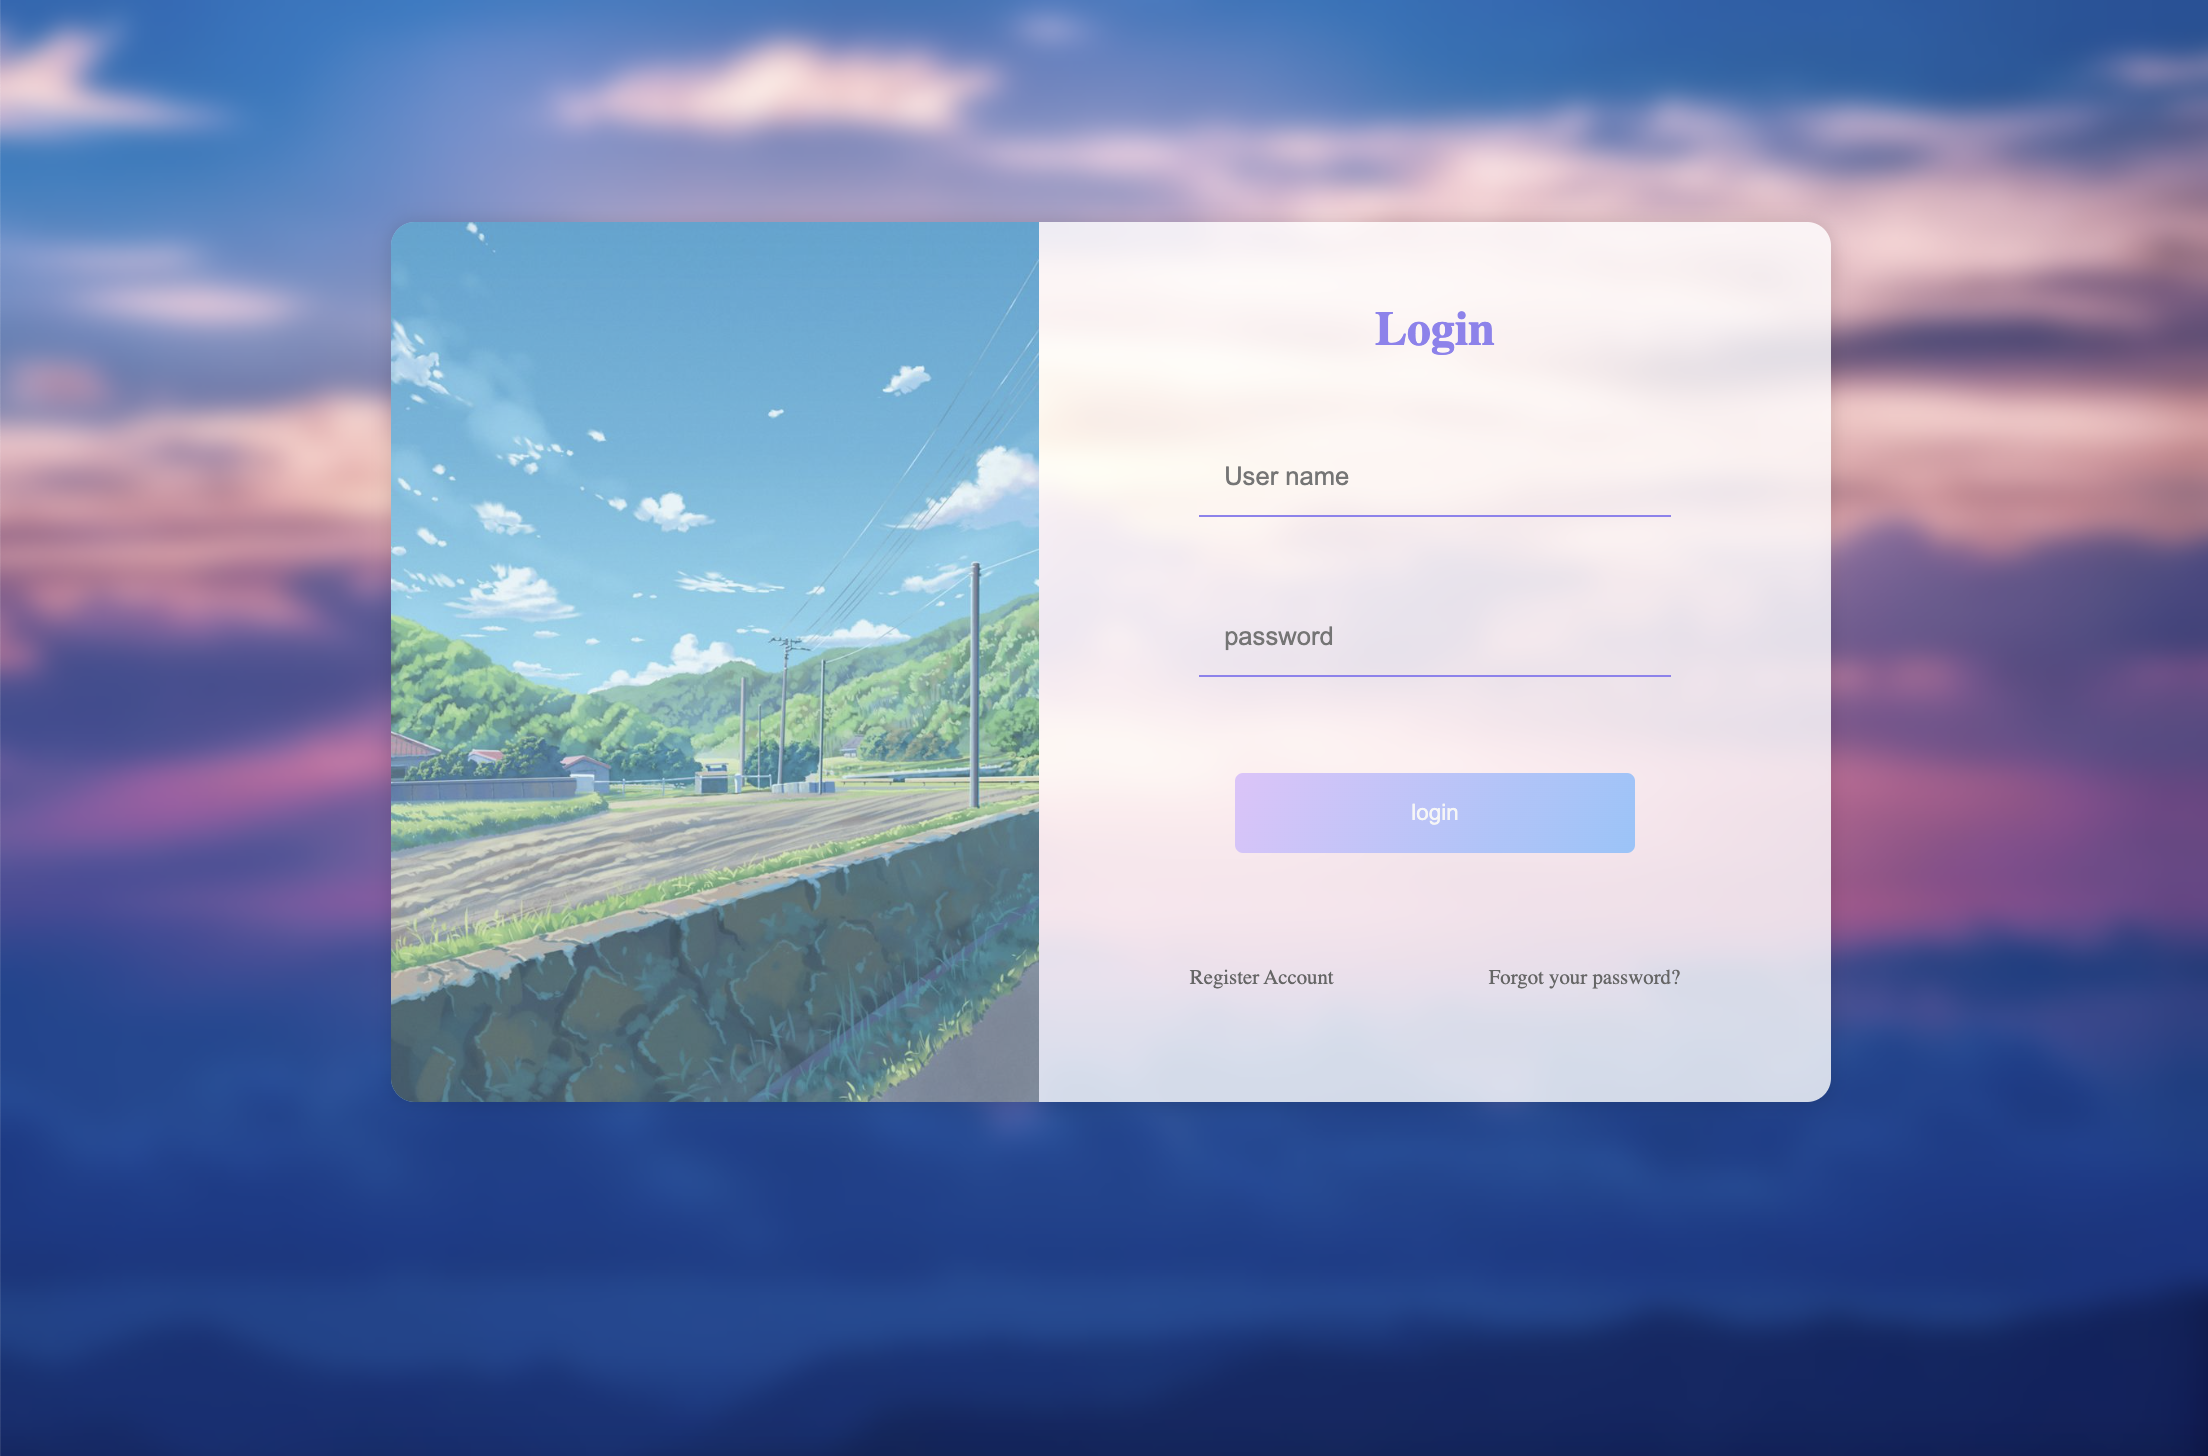
\includegraphics[width=1\linewidth]{login.png}
\caption{\label{login.png}login page}
\end{figure}

\begin{figure}
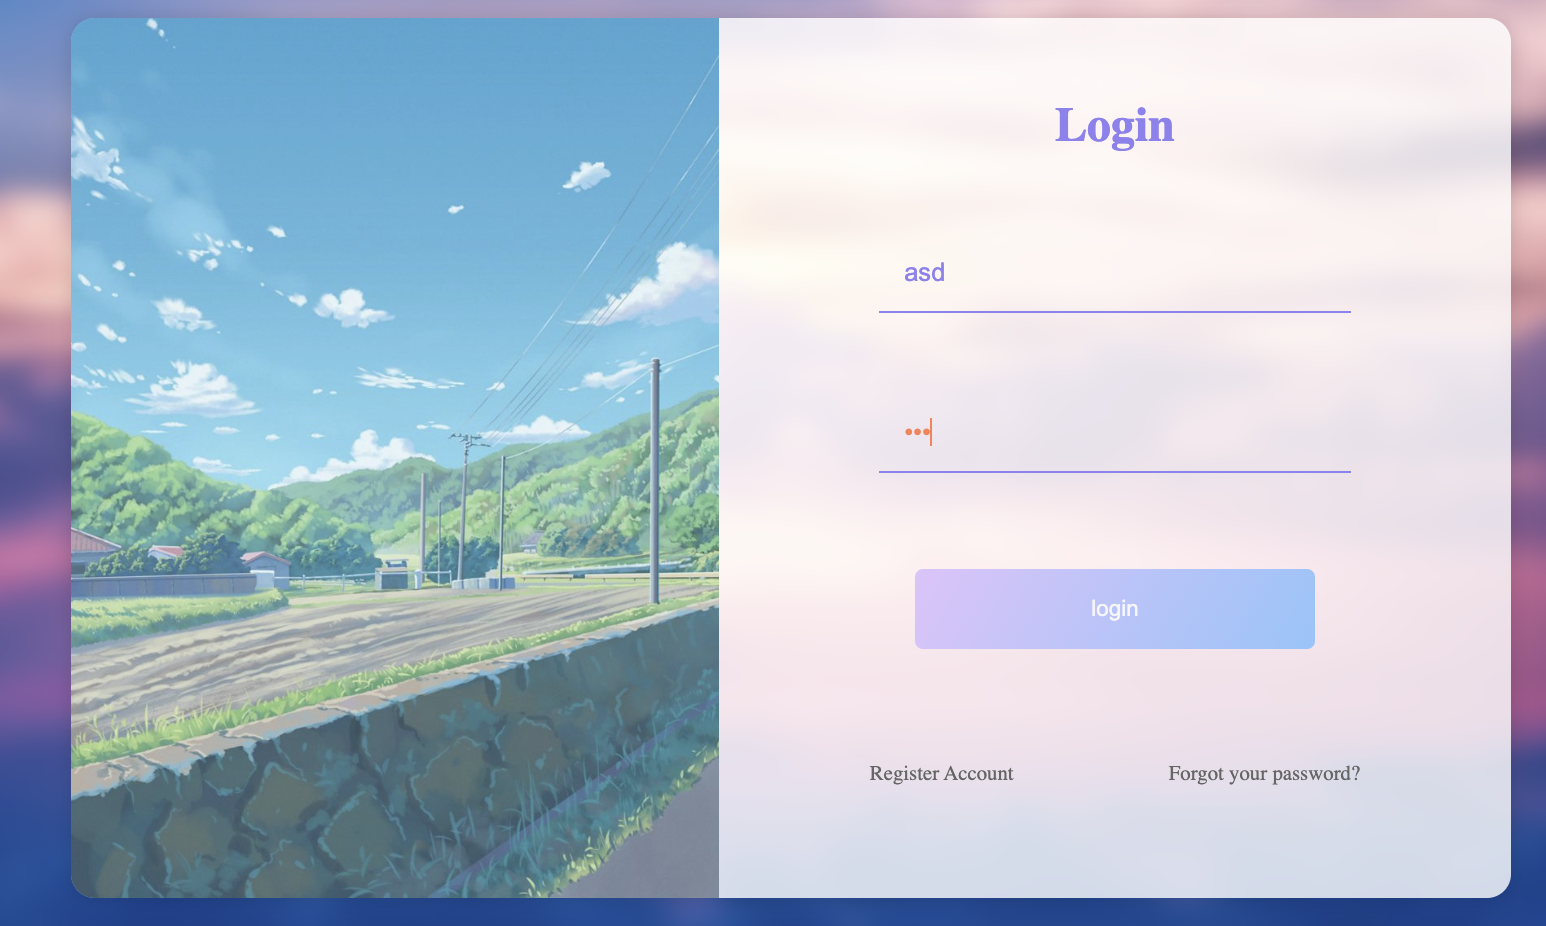
\includegraphics[width=1\linewidth]{login1.png}
\caption{\label{login1.png}Set username and password}
\end{figure}

\begin{figure}
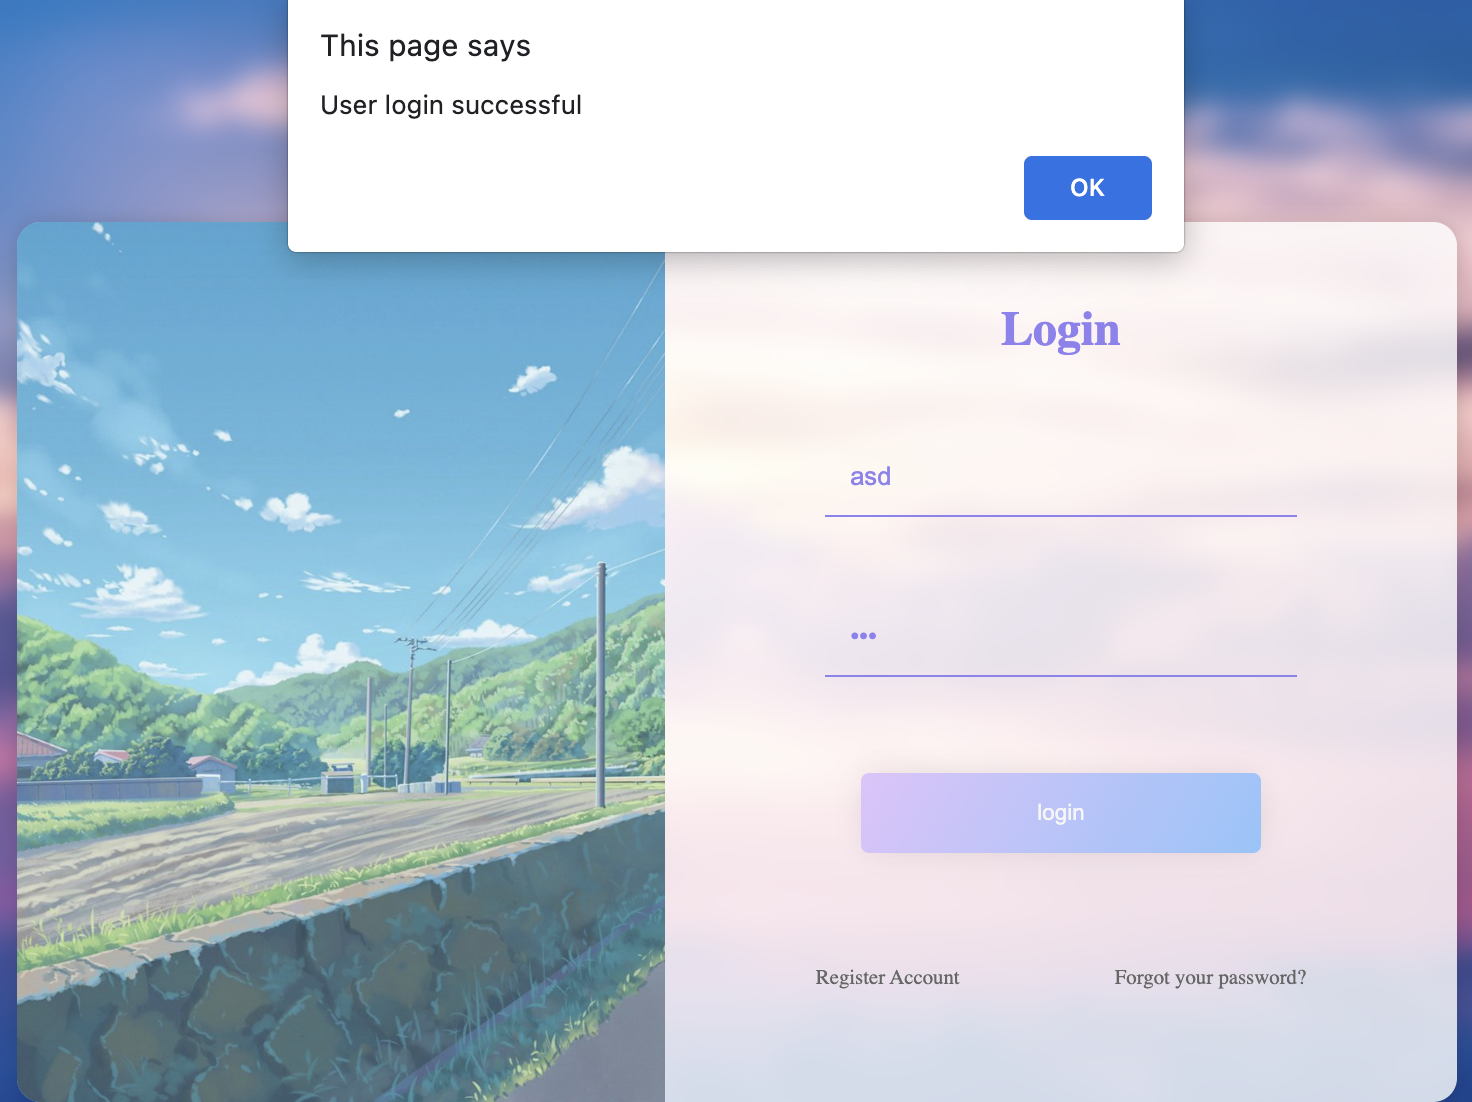
\includegraphics[width=1\linewidth]{login2.png}
\caption{\label{login2.png}Successful}
\end{figure}

\begin{figure}
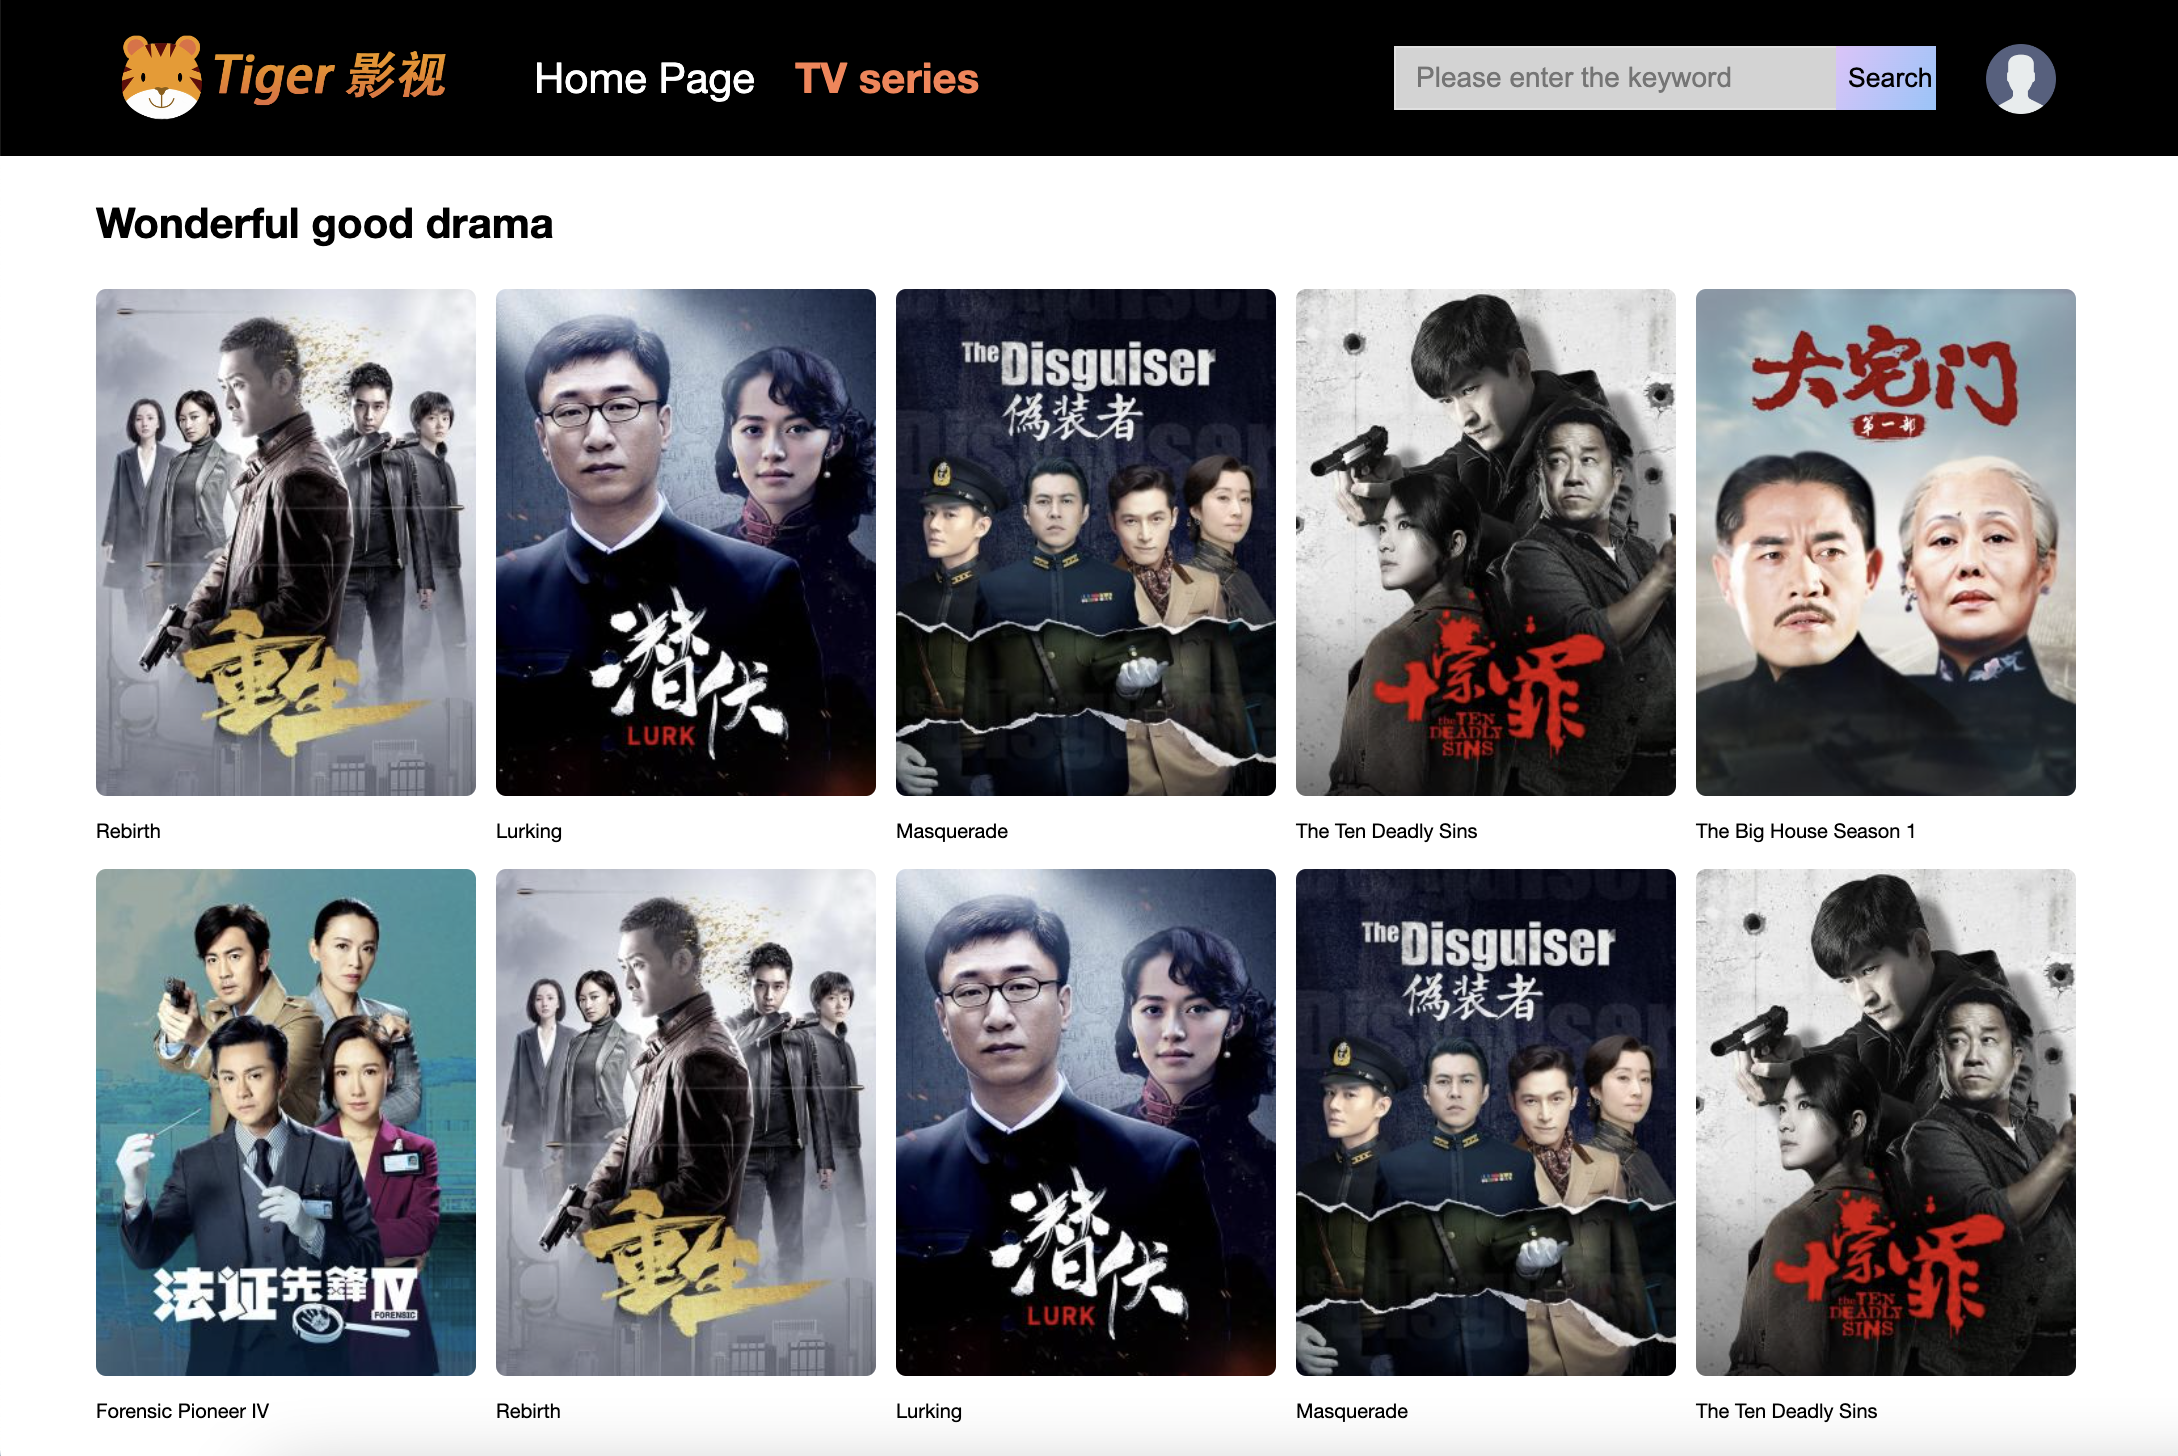
\includegraphics[width=1\linewidth]{hp.png}
\caption{\label{hp.png}Home page}
\end{figure}

\begin{figure}
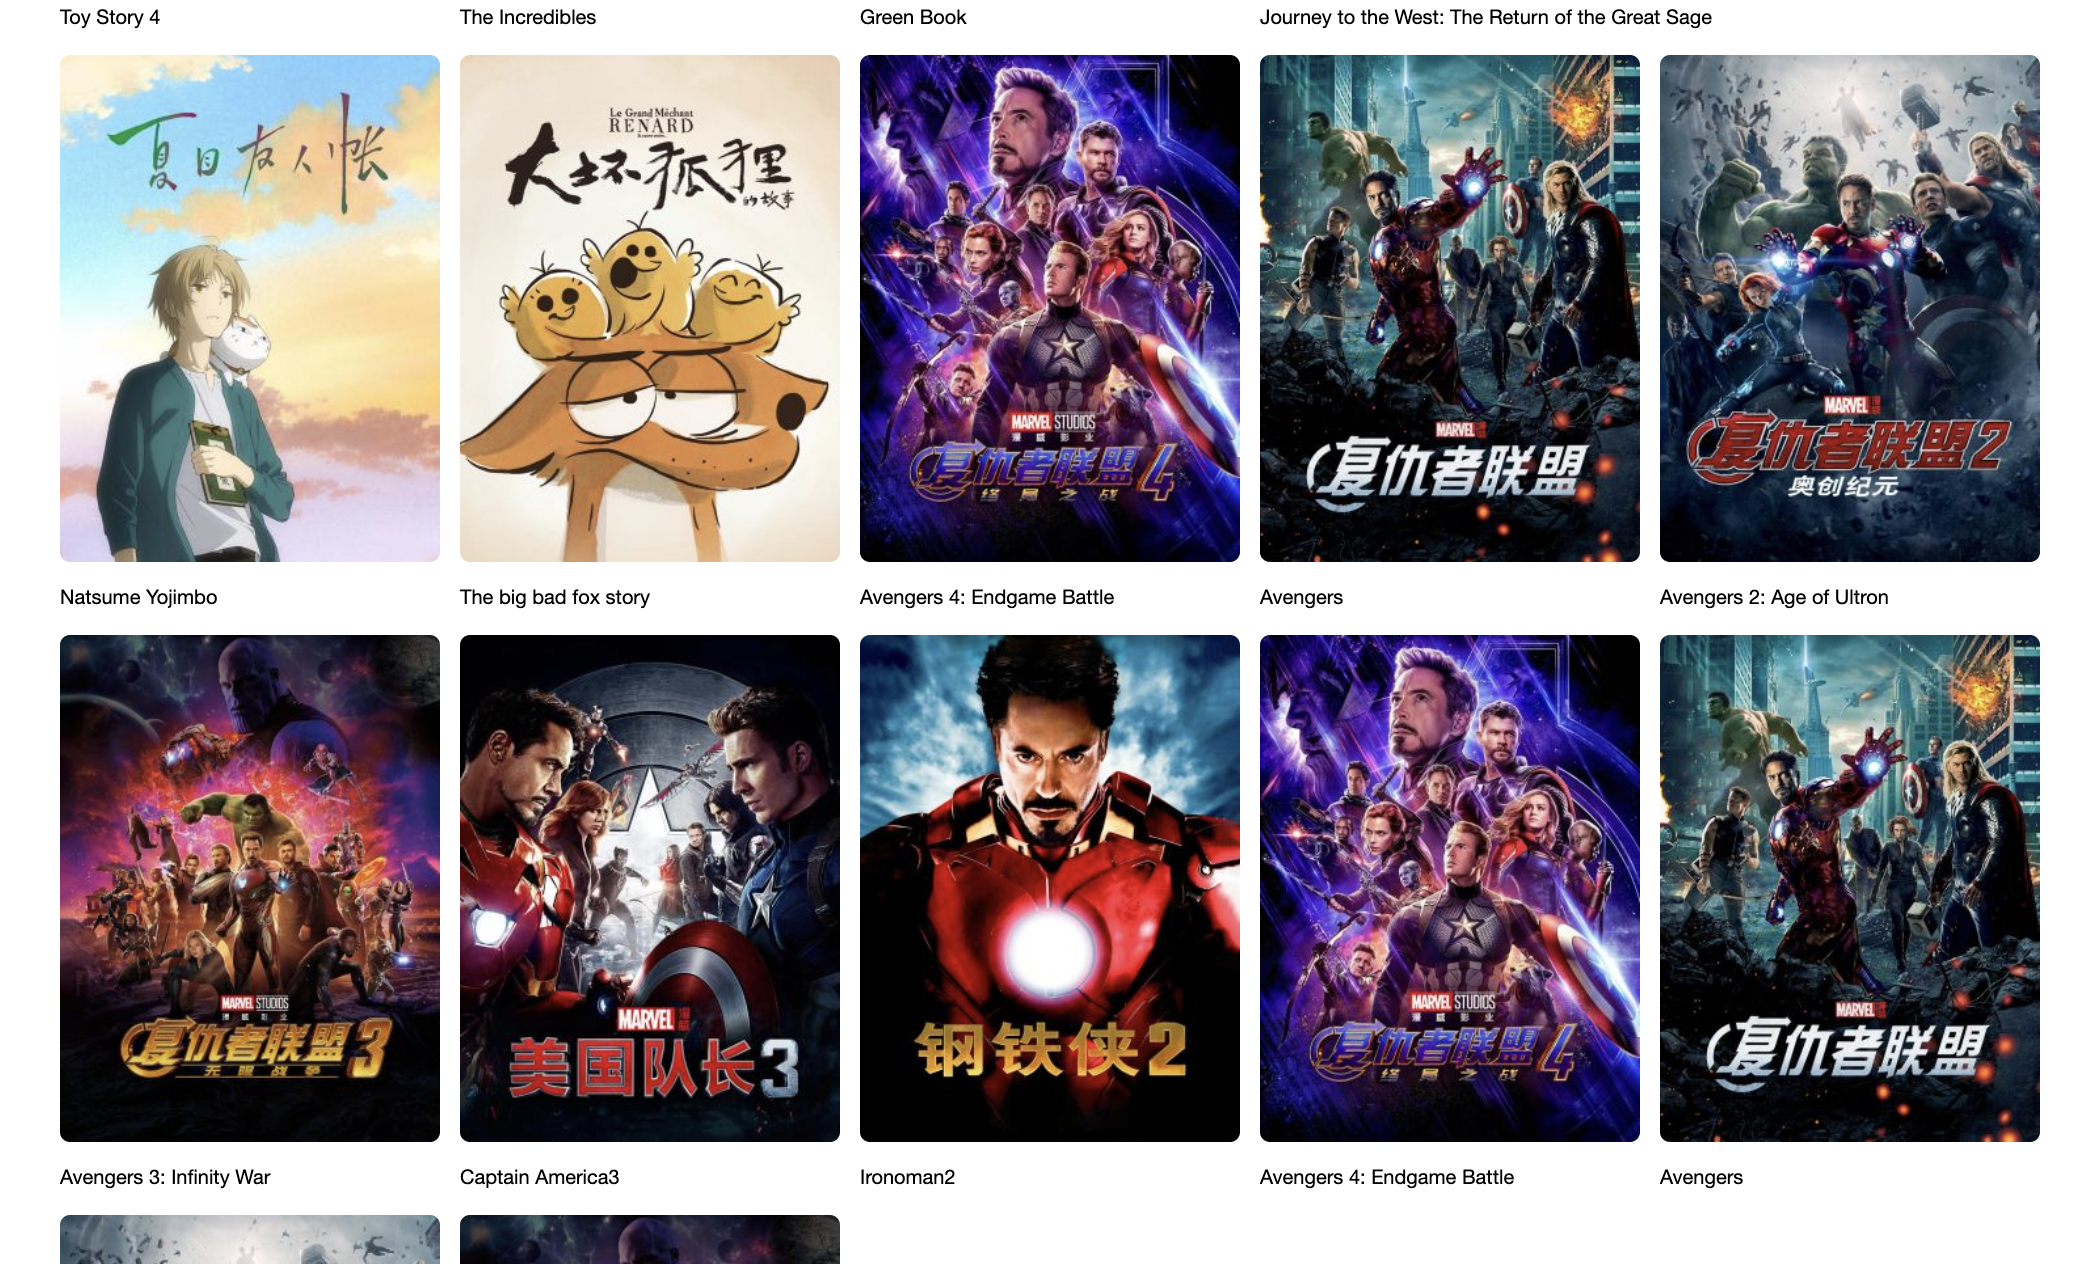
\includegraphics[width=1\linewidth]{hp1.png}
\caption{\label{hp1.png}Home page}
\end{figure}

\begin{figure}
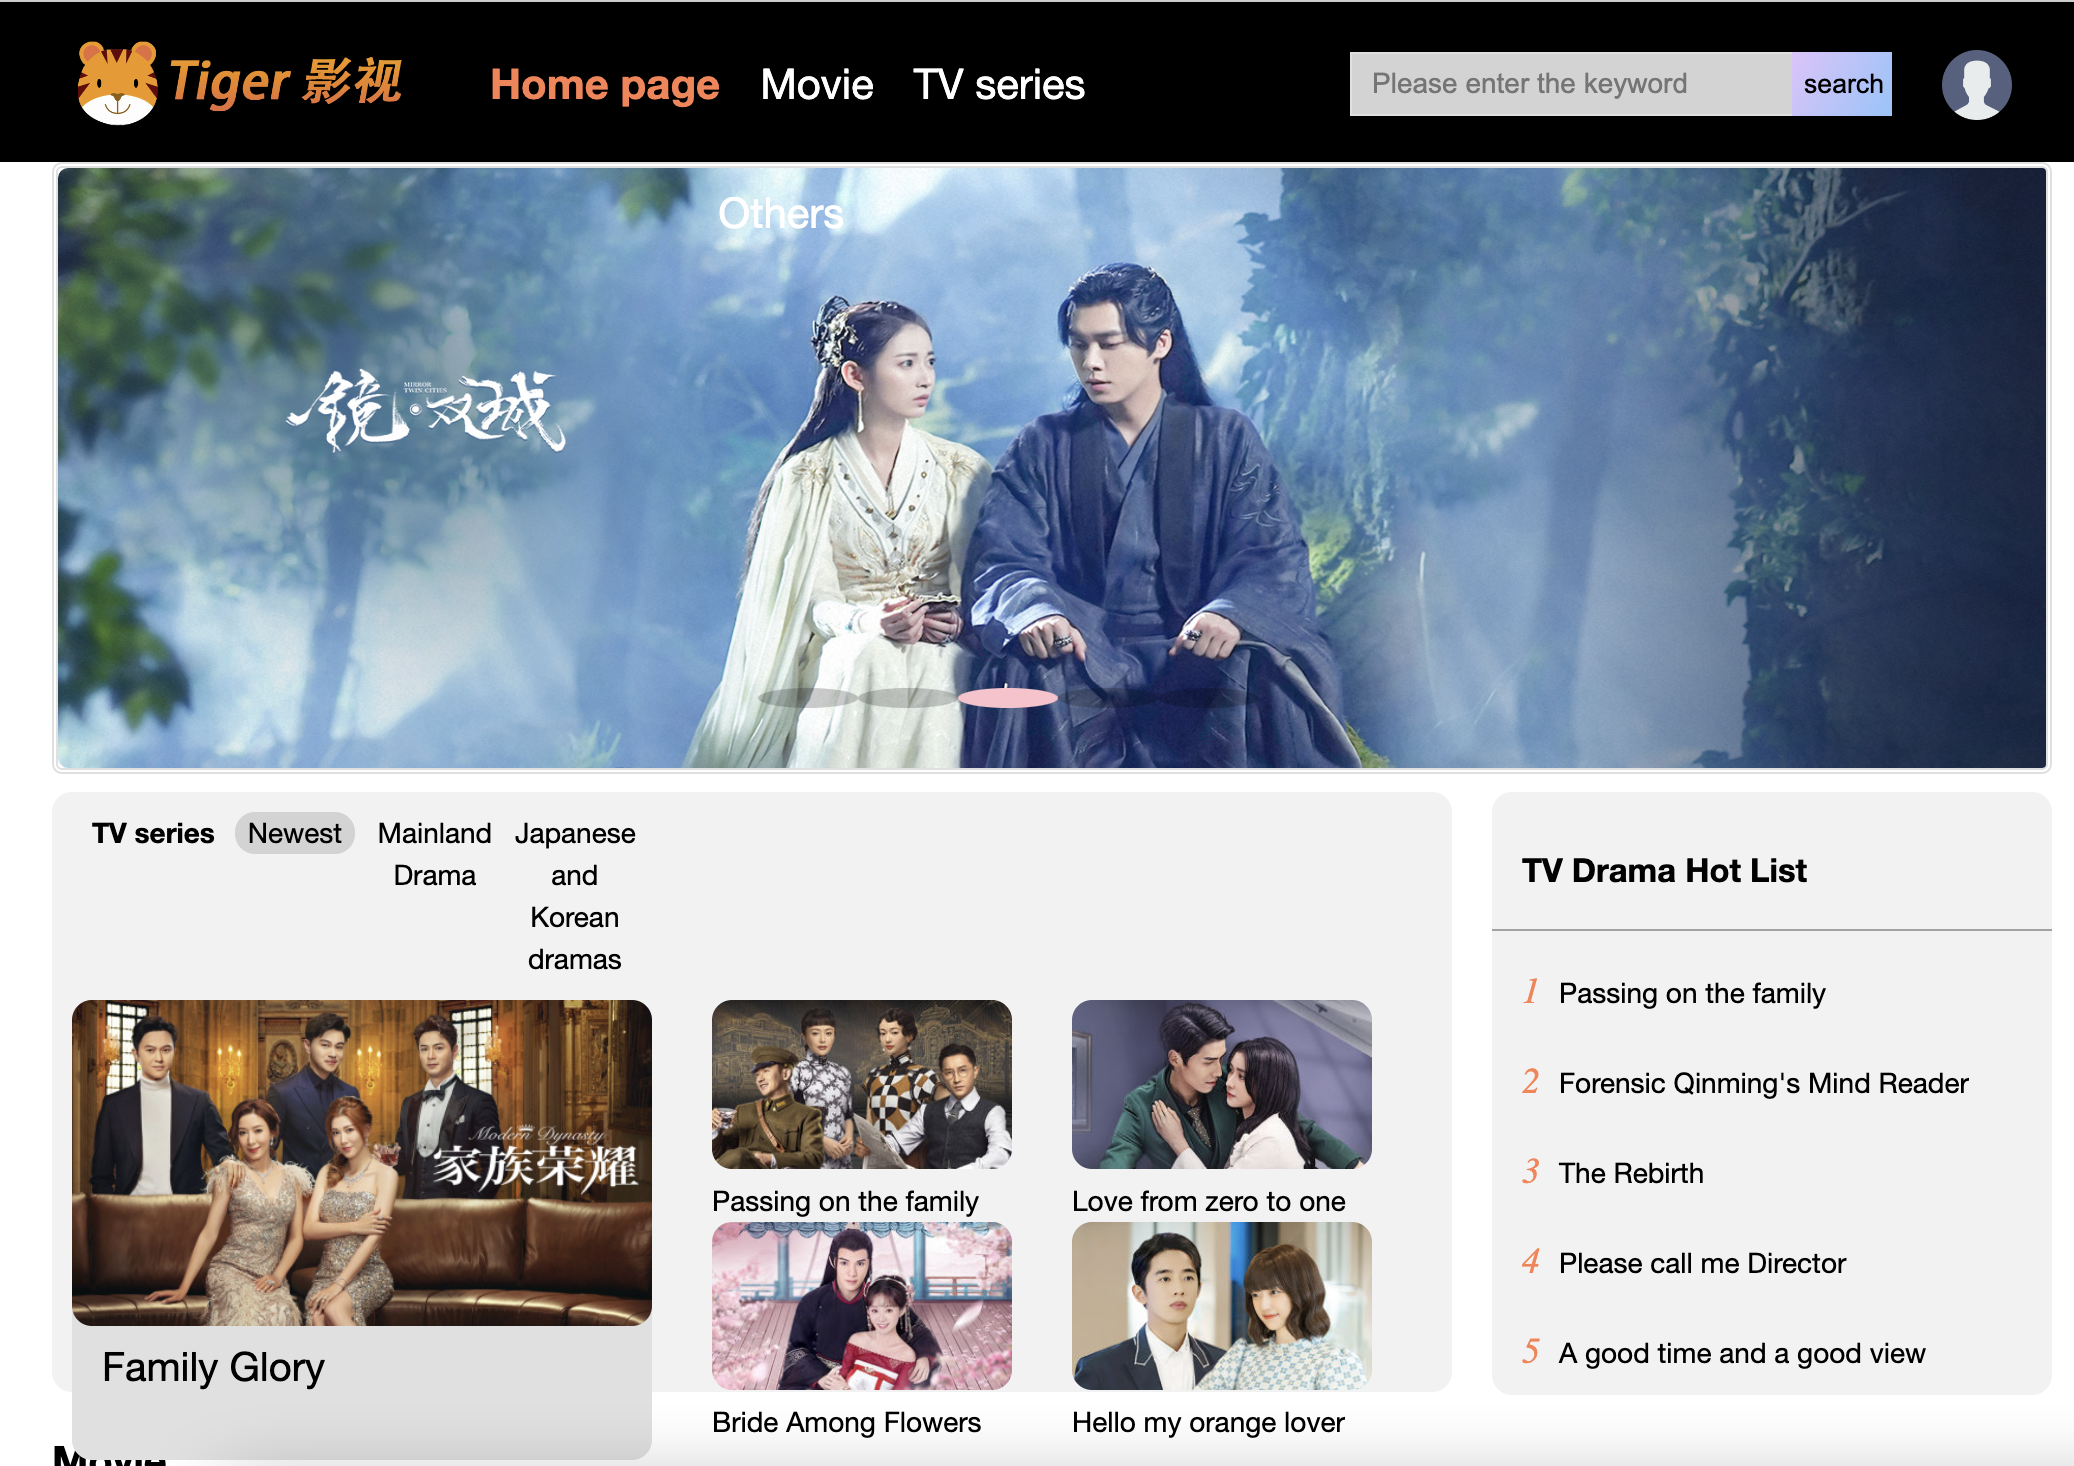
\includegraphics[width=1\linewidth]{hp2.png}
\caption{\label{hp2.png}Home page}
\end{figure}

\begin{figure}
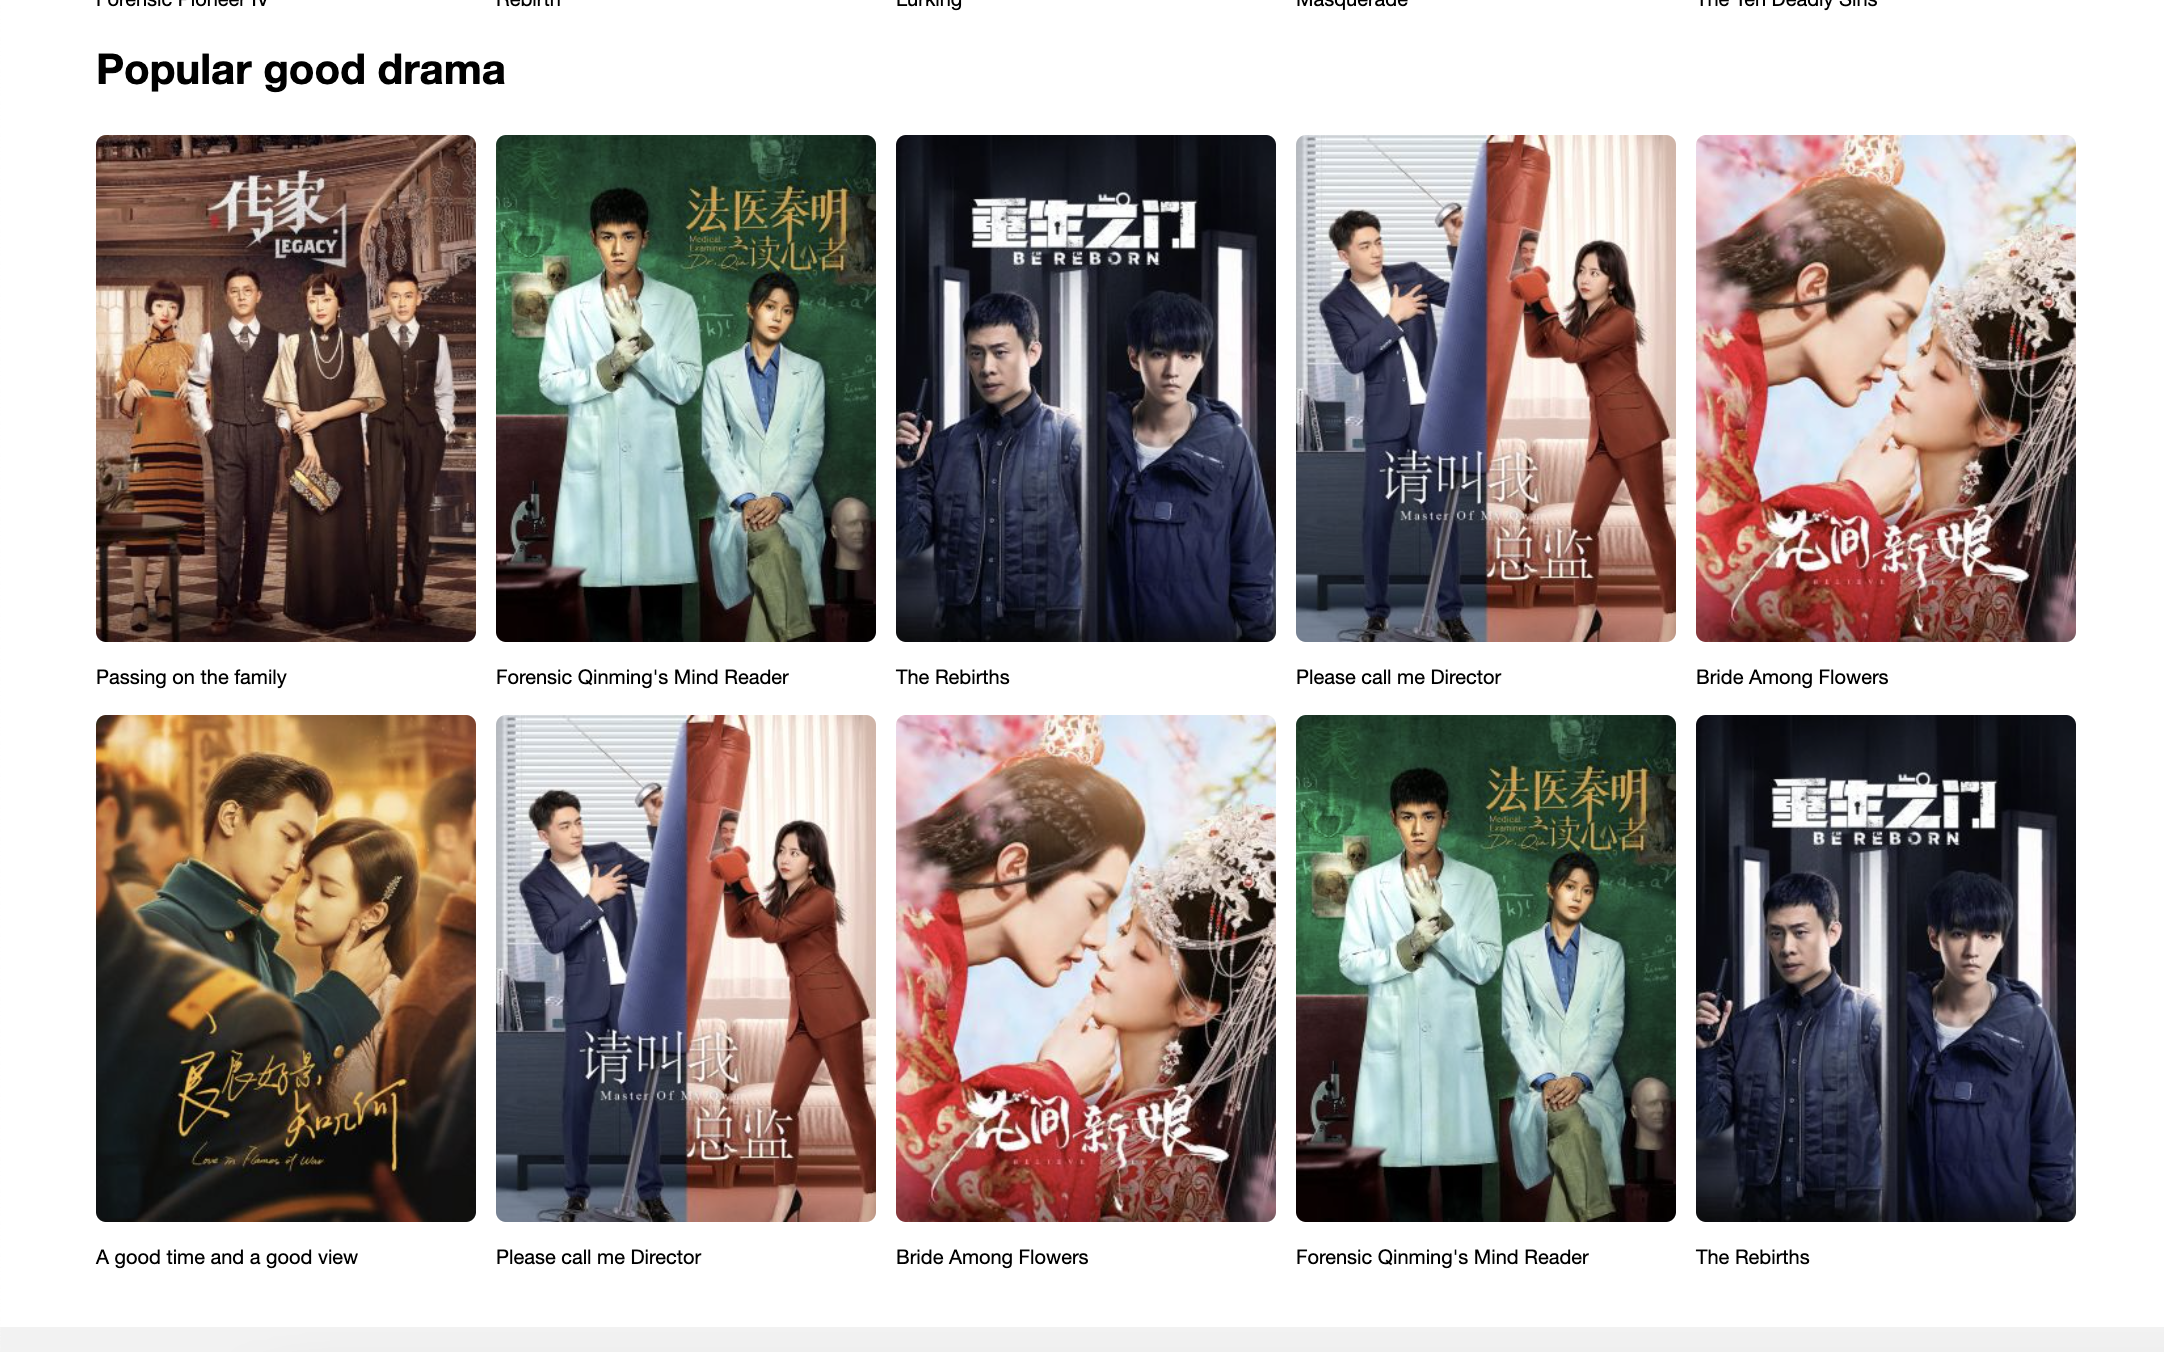
\includegraphics[width=1\linewidth]{index1.png}
\caption{\label{index1.png}Index page}
\end{figure}

\begin{figure}
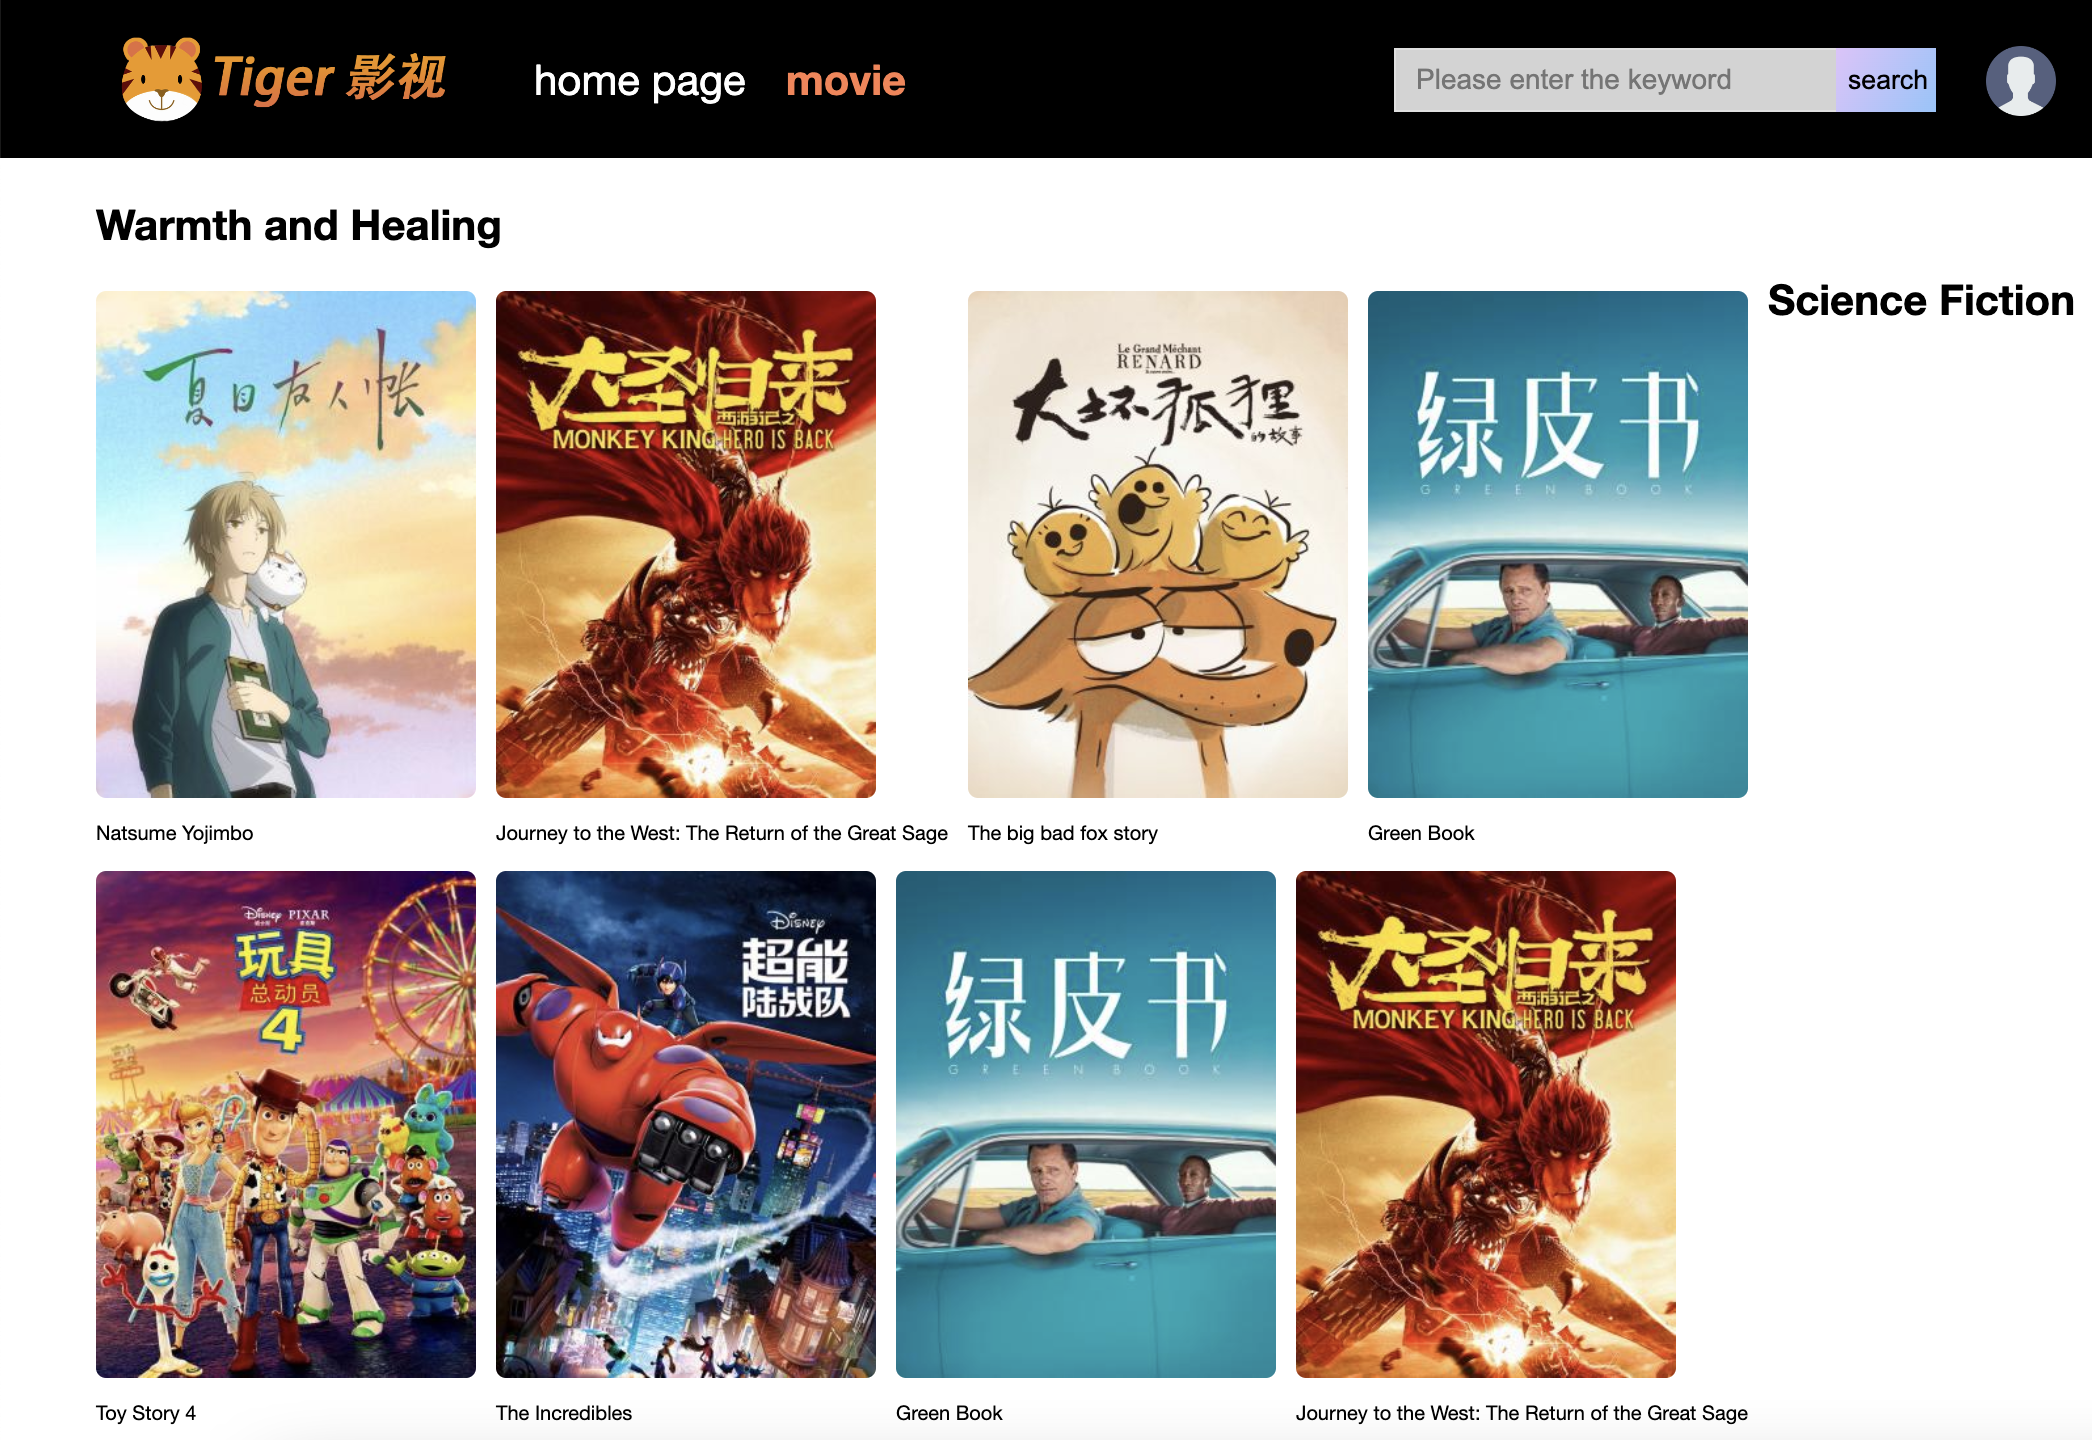
\includegraphics[width=1\linewidth]{index2.png}
\caption{\label{index2.png}Index page}
\end{figure}

\begin{figure}
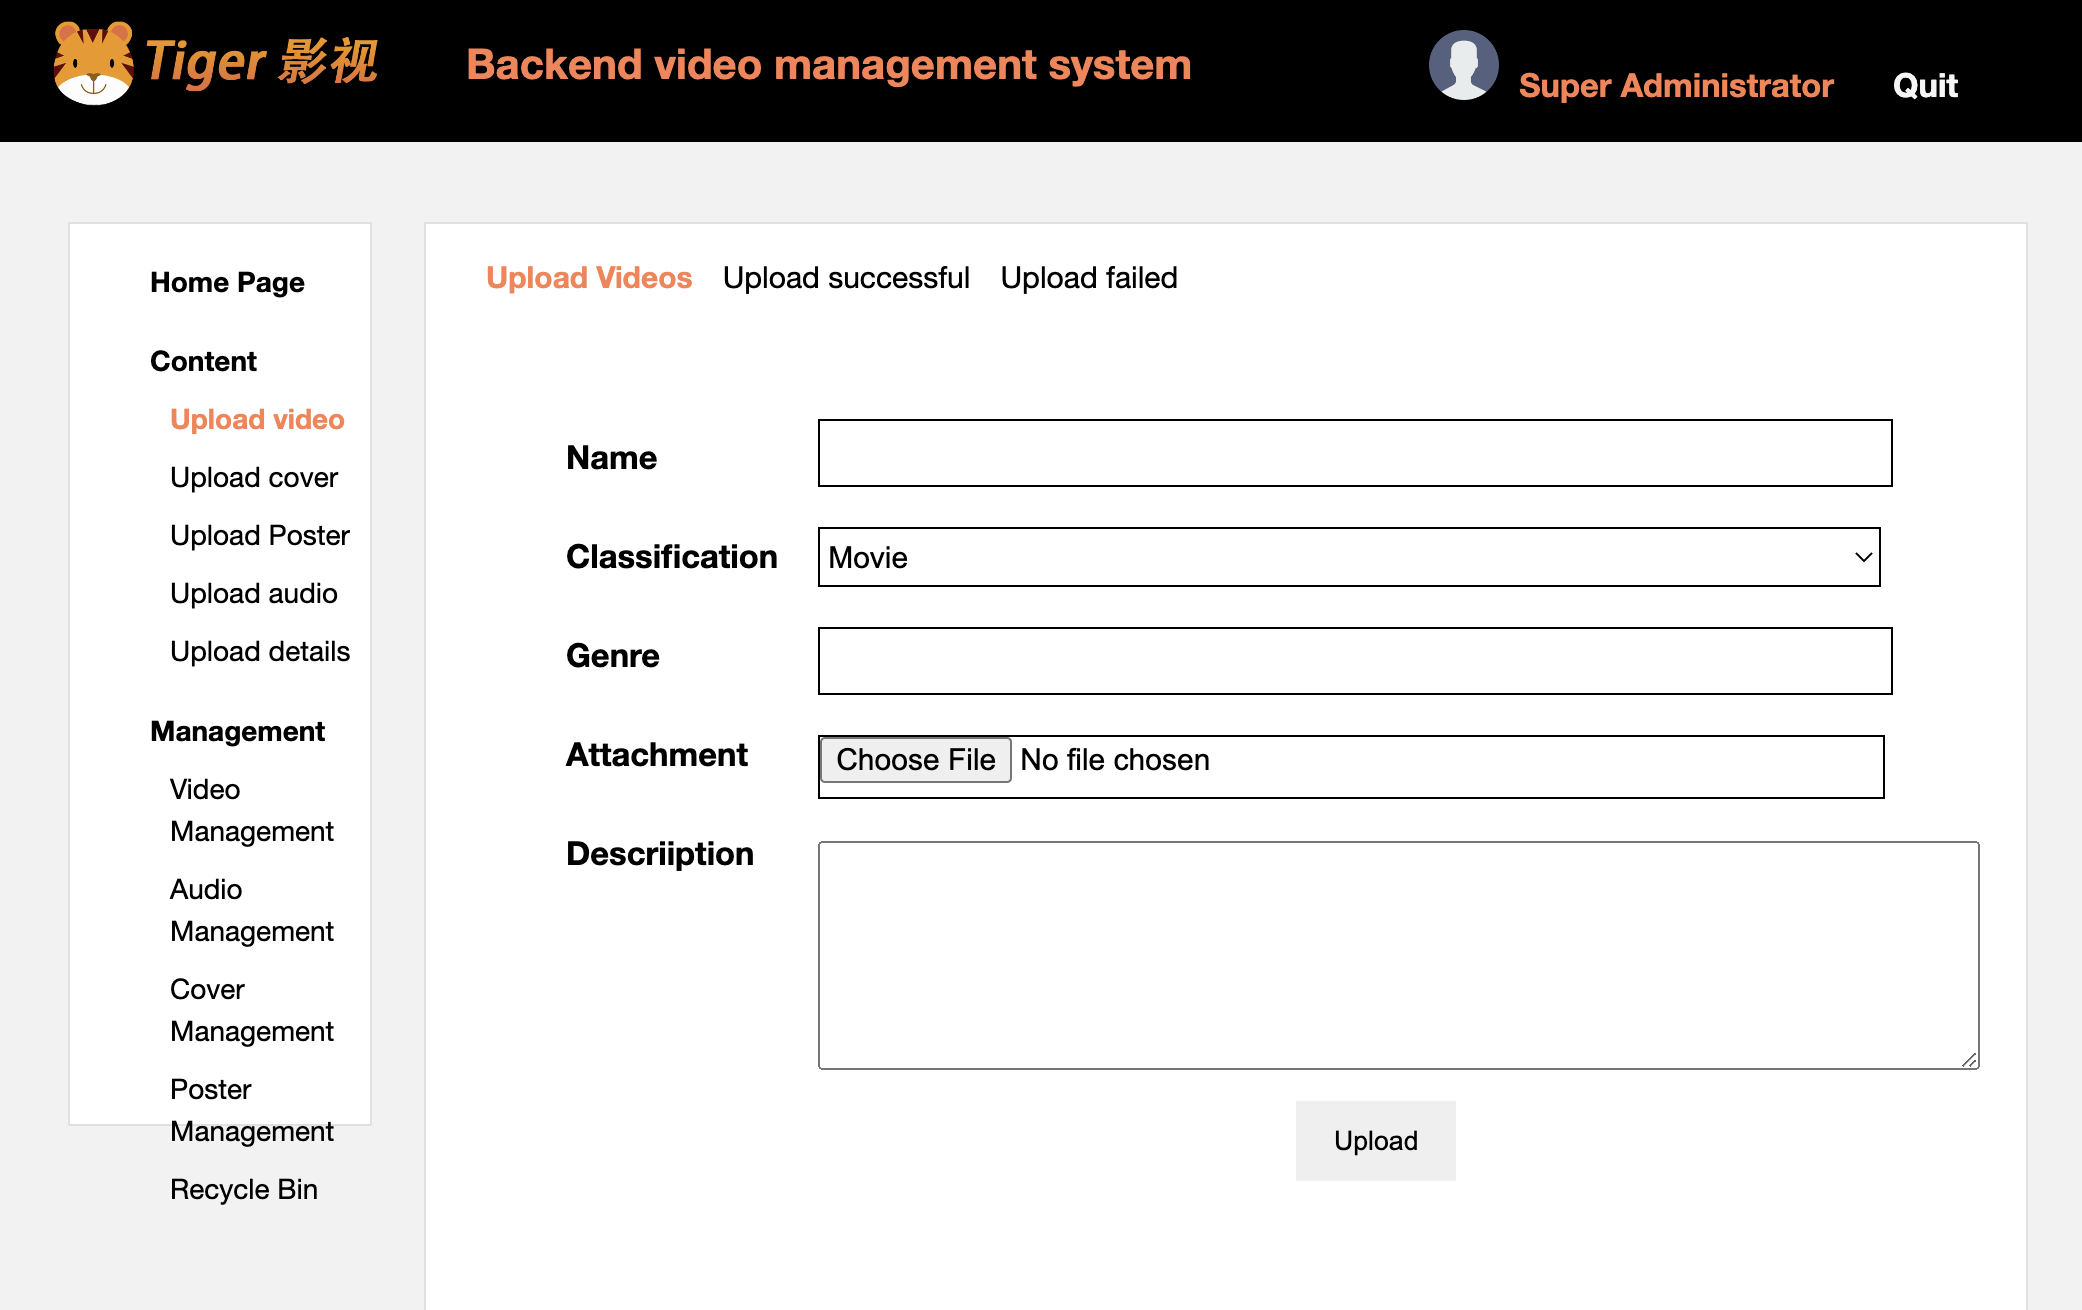
\includegraphics[width=1\linewidth]{mng.png}
\caption{\label{mng.png}management page}
\end{figure}
\subsection{Screenshots}



%=============================================================================

\newpage
\section{Level B: Basic Application}

Whilst level A is about doing something simple with the topic to just show that you have started to be able to use the tool or technology, level B is about doing something practical that might actually be useful.

\subsection{Level B Demonstration}
\begin{itemize}
\item User Inputs and Validation: The application accepts two user inputs. These could be a video title and a URL, for instance. Prior to processing these inputs, the application verifies their validity. This could involve checking the format of the URL or ensuring that the video title doesn't contain any disallowed characters. This demonstrates my understanding of form handling and input validation in JavaScript.

\item Data Handling and Display: Upon validation, the application stores the video and its associated URL. It juxtaposes the descriptions in a list, which indicates an understanding of data storage and manipulation in JavaScript. Most likely,  I am using some form of data structure (like an array or an object) to store these entries.

\item Dynamic Updating of User Interface: The application displays the most recent record at the top of the list. This involves dynamically updating the user interface based on the state of the data, a fundamental concept in JavaScript web development.

Data Clearing Functionality: I've included a button to clear the data. This demonstrates my understanding of event handling in JavaScript, as well as the ability to manipulate and reset the data stored by your application.
\end{itemize}
The code review would likely involve examining my approach to these features, how I've organized your code across multiple pages, and my overall JavaScript, HTML, and CSS skills. Some areas of focus might include my data validation techniques, how I're storing and retrieving data, my methods for updating the user interface, and my event handling for the data clearing button.

\subsection{Application artifacts}

My application is a multi-page web program built to catalog and display videos based on user input. It's a simple yet functional JavaScript application demonstrating essential web development skills.

Functionality:
The program prompts the user for two inputs on each page. One could be the video title and the other could be the corresponding URL. After the user enters these details, the application verifies if the input is valid. It could check, for instance, that the URL is in the correct format and the video title doesn't include disallowed characters or is not already present in the list.

Upon successful validation, the application adds the video and its URL to a list. The list juxtaposes the description of the videos, providing a neat, organized view of the collected data. Each new video entry is added to the top of the list, allowing users to quickly view the most recent additions.

Additionally, the application features a clear button that, when clicked, erases all the data from the list. This functionality provides users with a simple way to start afresh.

Implementation:
The application was created using HTML, CSS, and JavaScript. HTML was used to structure the web pages and create the necessary input fields, buttons, and list display. CSS was used to style these elements and provide a visually pleasing and easy-to-navigate user interface.

JavaScript played a key role in adding interactivity to the application. Functions were written to capture user inputs, perform validation checks, add valid entries to the list, display the list on the page, and clear the list when required. The list data may have been stored in a JavaScript array or object, and the Document Object Model (DOM) was used to manipulate the webpage based on this data. As the user provides new input or chooses to clear the data, JavaScript updates the display in real time, demonstrating the dynamic nature of web applications.

\subsection{Screenshots}
\begin{figure}
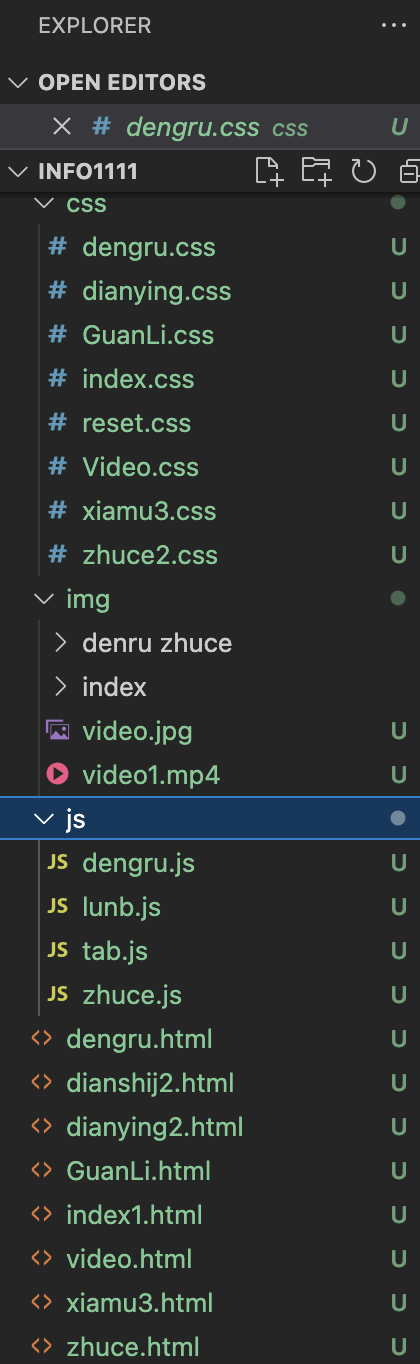
\includegraphics[width=0.4\linewidth]{main frame html.png}
\caption{\label{main frame html.png}set main frame}
\end{figure}

\begin{figure}
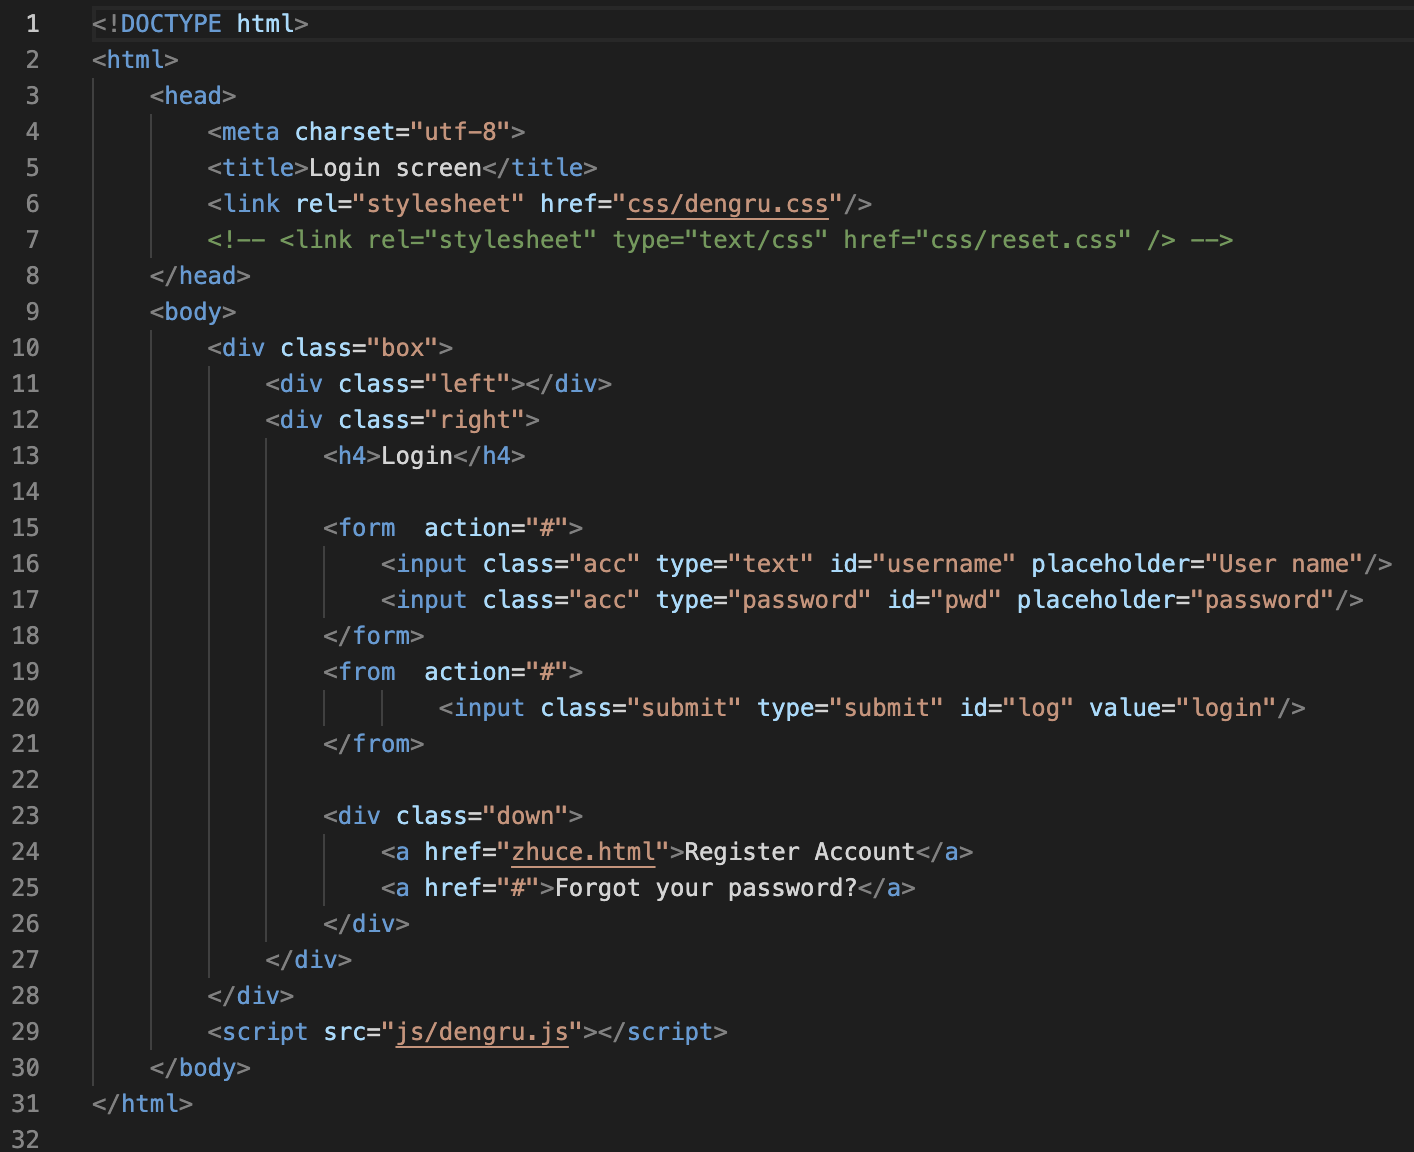
\includegraphics[width=1\linewidth]{login file html.png}
\caption{\label{login file html.png}complete login function in html}
\end{figure}

\begin{figure}
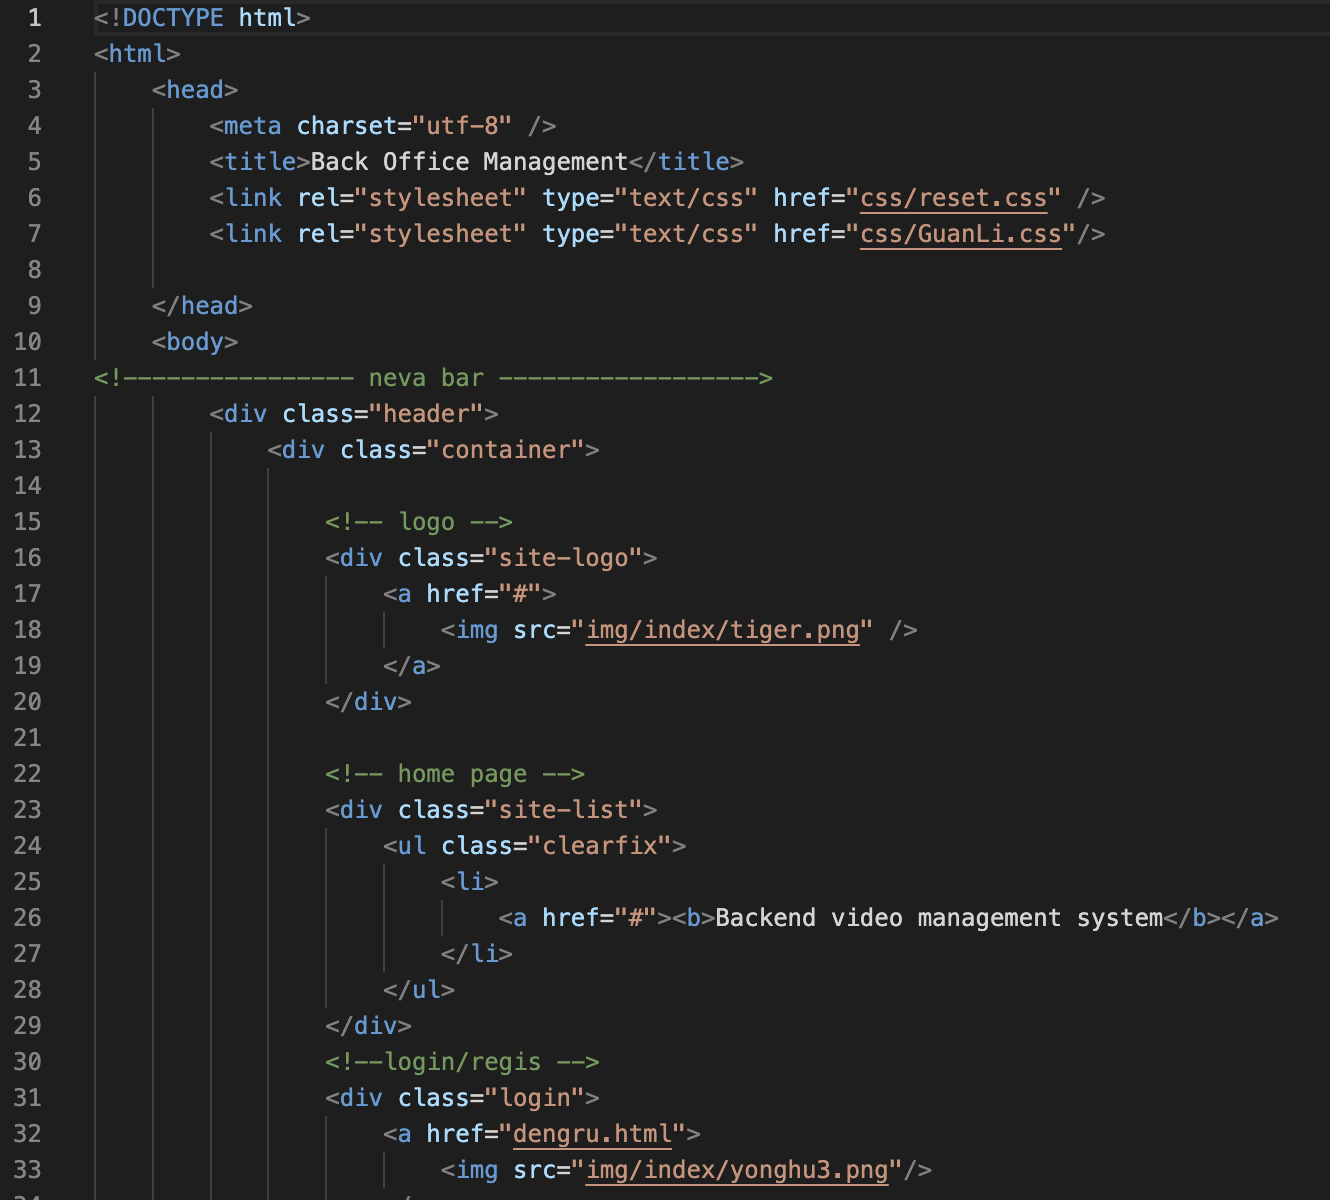
\includegraphics[width=1\linewidth]{management file htaml.png}
\caption{\label{management file htaml.png}complete management file in html}
\end{figure}

\begin{figure}
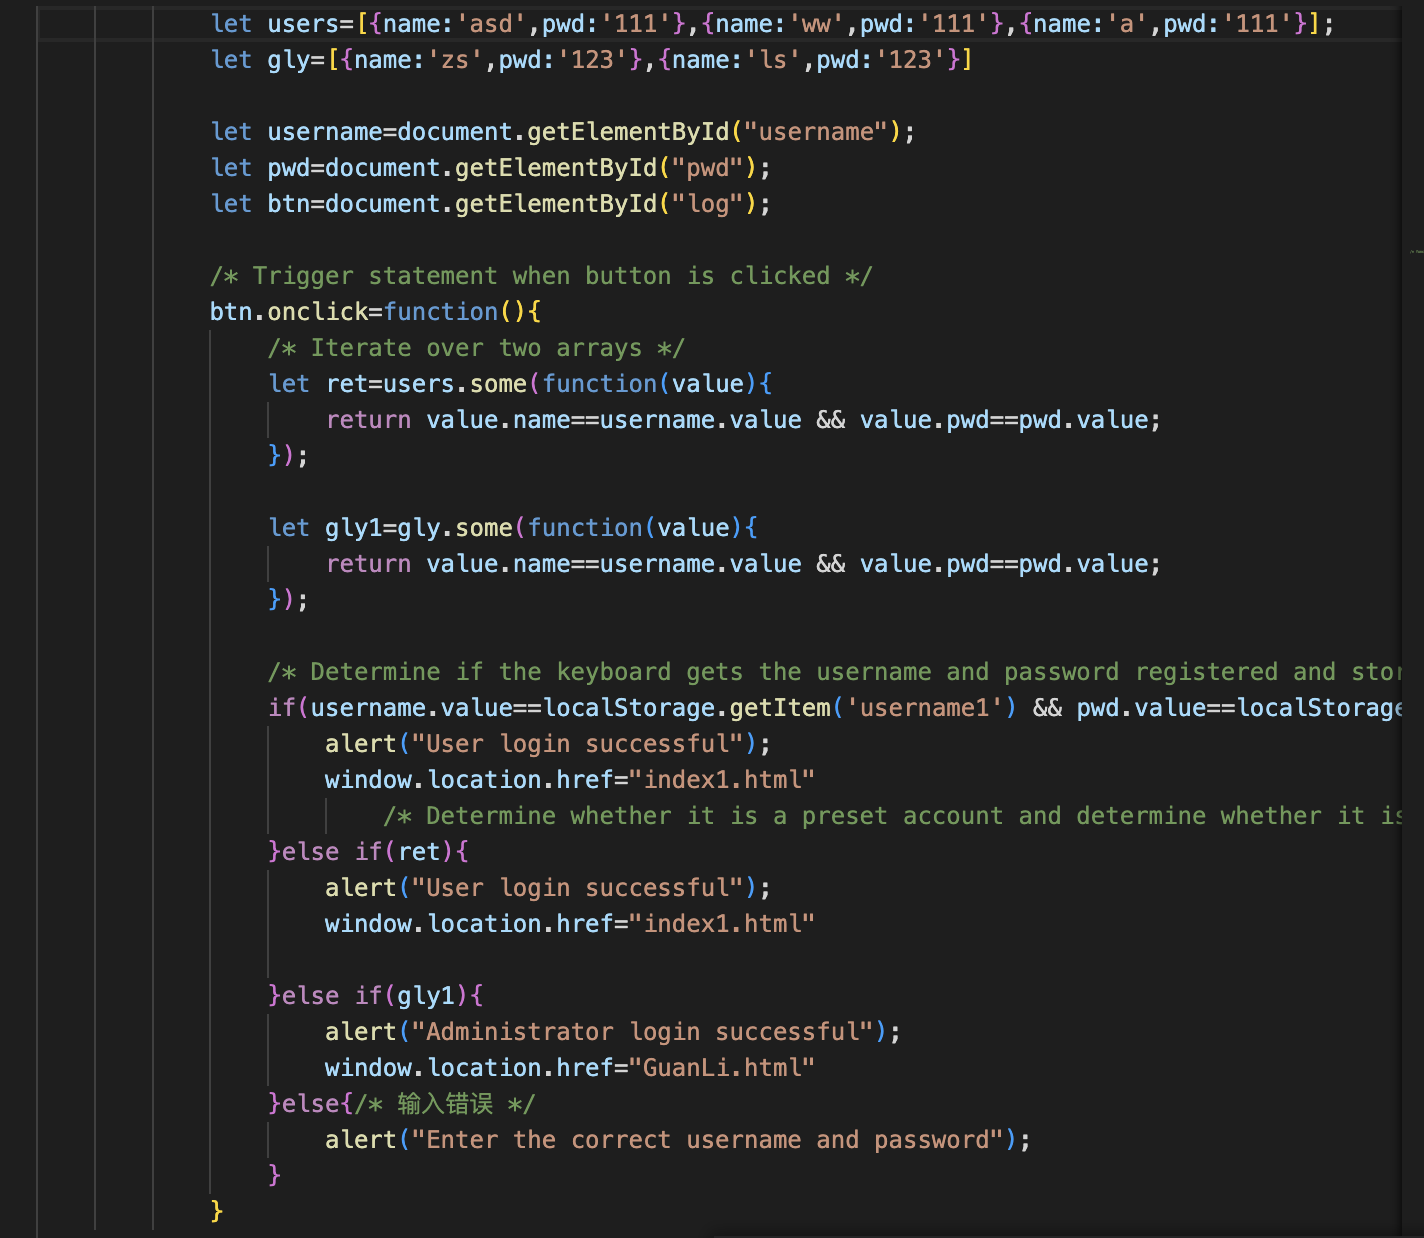
\includegraphics[width=1\linewidth]{login file javascript.png}
\caption{\label{login file javascript.png}complete login file in js}
\end{figure}

\begin{figure}
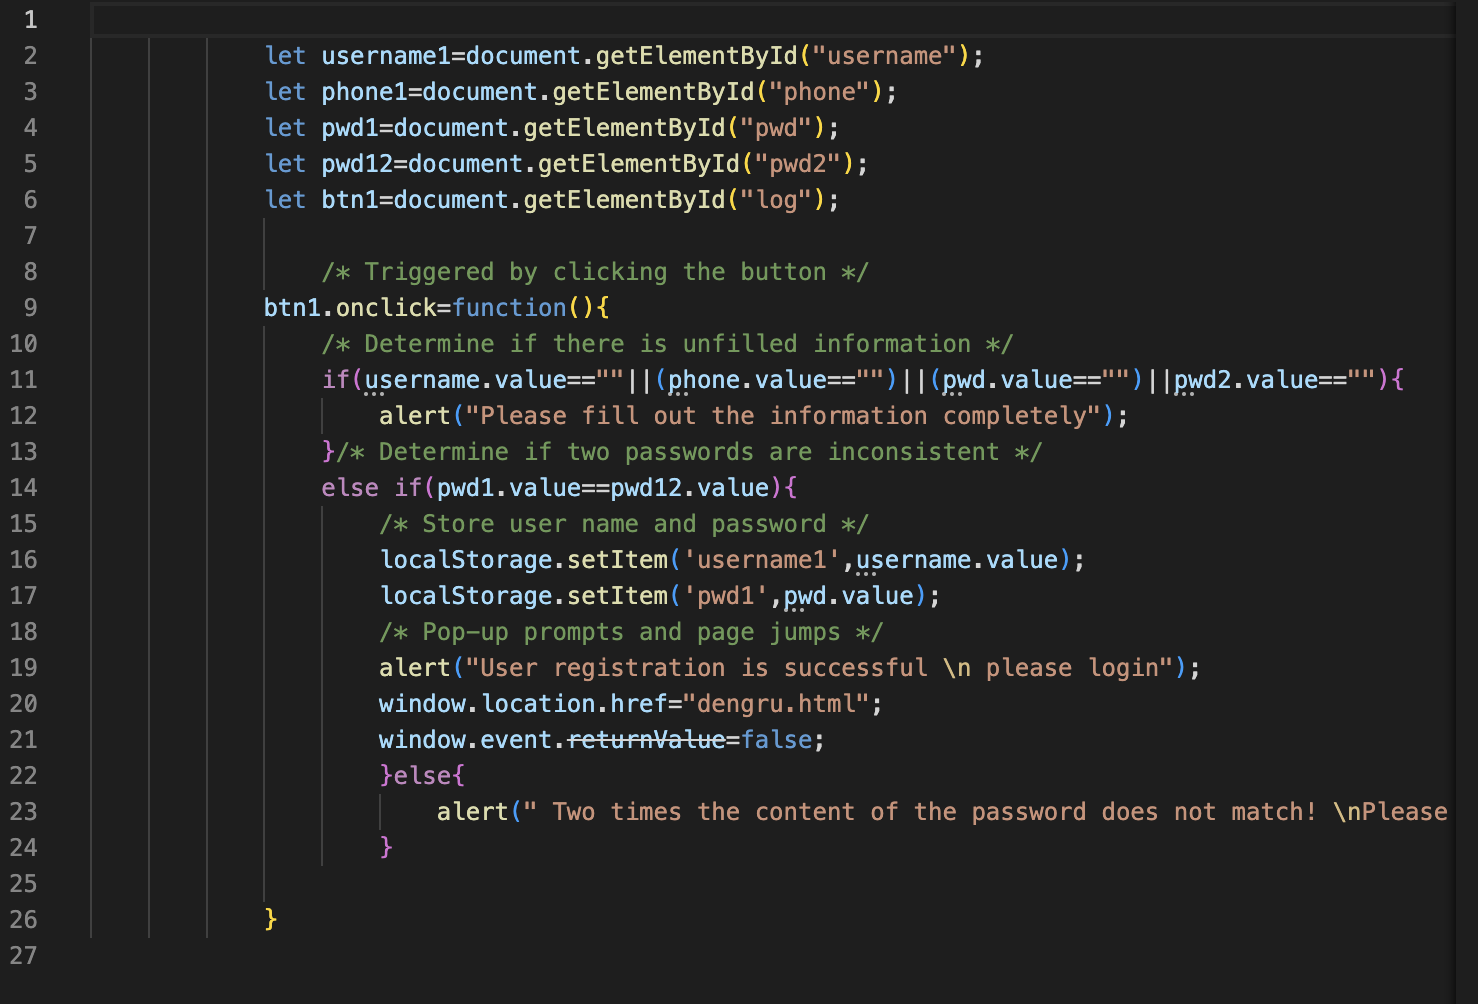
\includegraphics[width=1\linewidth]{register file javascript.png}
\caption{\label{register file javascript.png}complete register file in js}
\end{figure}

\newpage
\subsection{Screenshots}
\begin{figure}
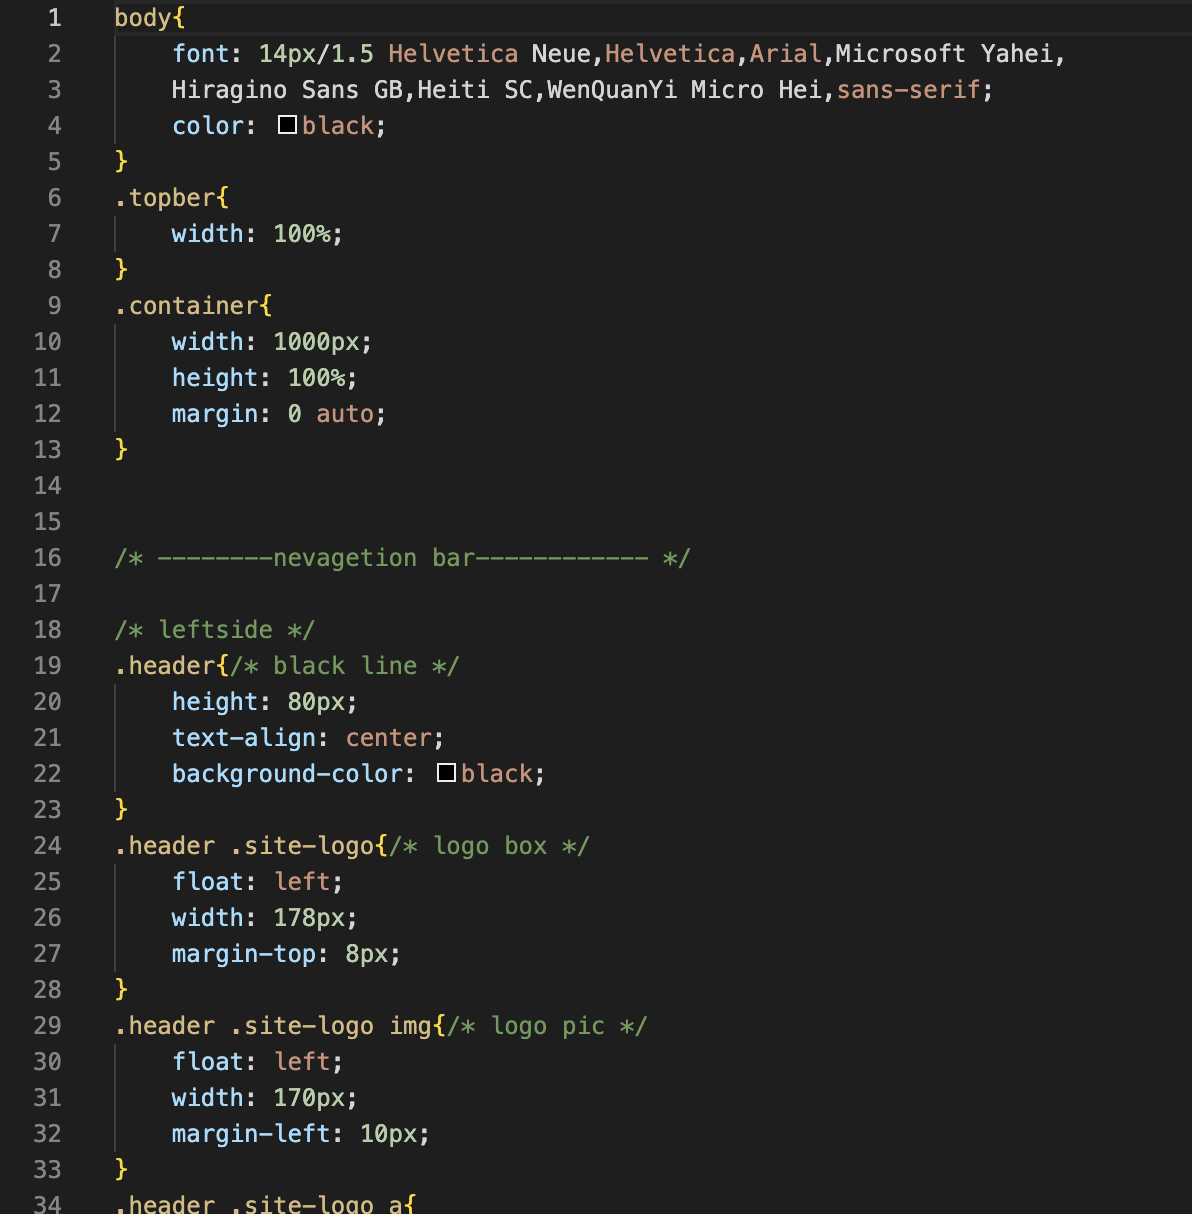
\includegraphics[width=1\linewidth]{index file css.png}
\caption{\label{index file css.png}complete index file in css}
\end{figure}

\begin{figure}
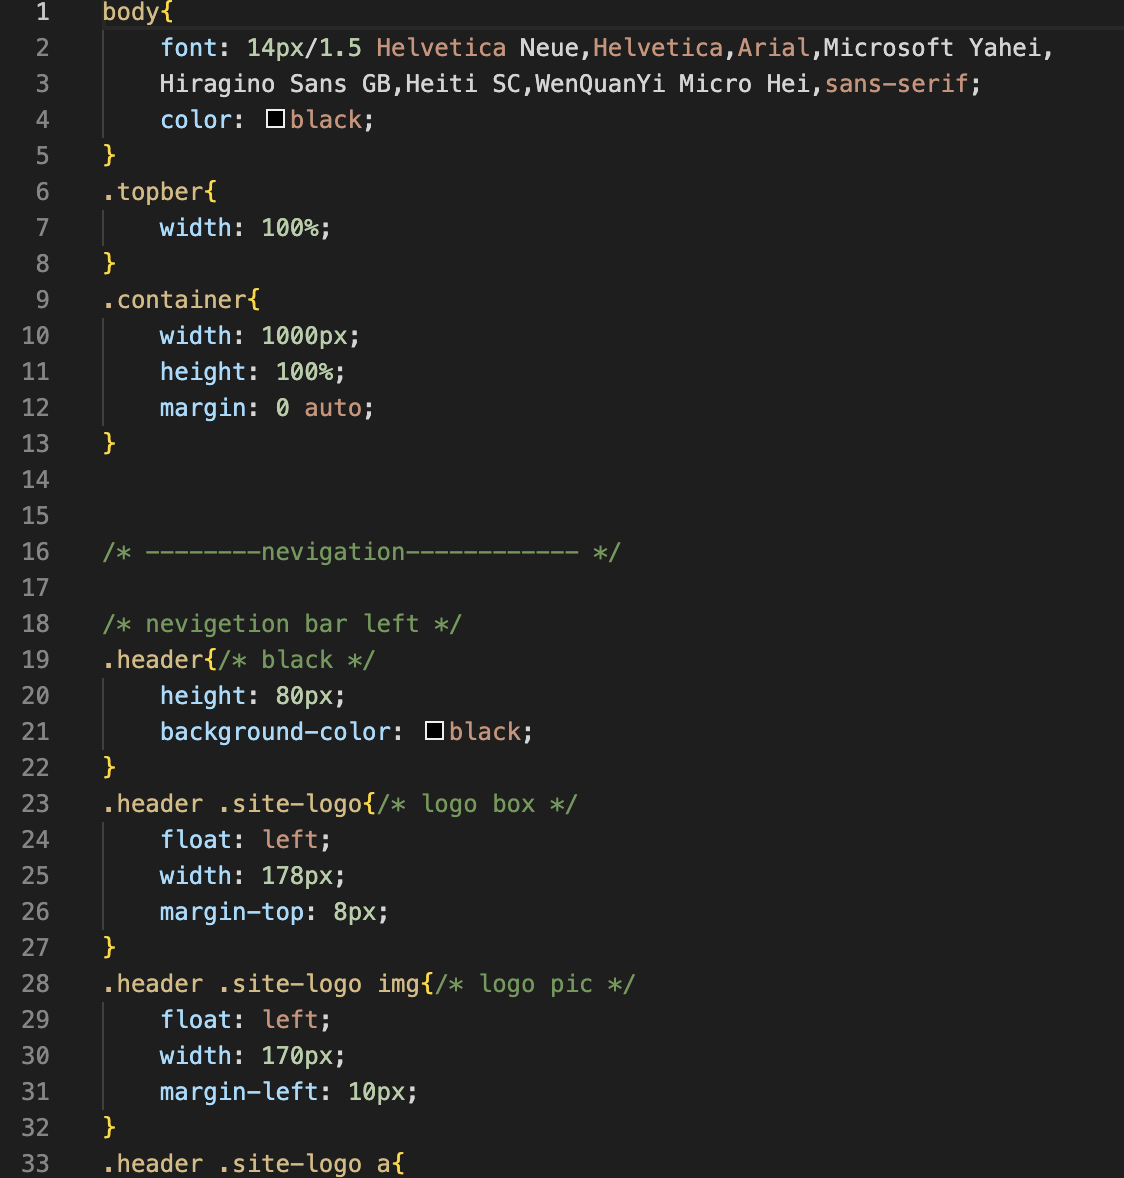
\includegraphics[width=1\linewidth]{movie file css.png}
\caption{\label{movie file css.png}complete movie file in css}
\end{figure}



%=============================================================================

\newpage
\section{Level C: Deeper Understanding}

Level C focuses on showing that you have actually understood the tool or technology at a relatively advanced level. You will need to compare it to alternatives, identifying key strengths and weaknesses, and the areas where this tool is most effective. 

\subsection{Strengths}
HTML, CSS, and JavaScript are three essential technologies used in web development. I have learned that they have those advantages:
HTML (Hypertext Markup Language):
\begin{itemize}
\item 	Structure: HTML provides the foundation for structuring web content. It allows you to define the hierarchy of elements, such as headings, paragraphs, lists, tables, forms, and more. This structural markup is crucial for organizing and presenting information on web pages.
\item 	Accessibility: HTML supports semantic tags, which give meaning to the content and help improve accessibility. By using appropriate semantic tags like <header>, <nav>, <main>, and <footer>, you make your website more accessible to assistive technologies and improve search engine optimization (SEO).
\end{itemize}
CSS (Cascading Style Sheets):
\begin{itemize}
\item 	Visual Styling: CSS allows you to control the visual presentation of HTML elements. With CSS, you can define colors, fonts, layouts, backgrounds, borders, and other visual properties of your web pages. It gives you the power to create visually appealing and consistent designs across your website.
\item 	Responsive Design: CSS enables responsive web design, which ensures that web pages adapt to different screen sizes and devices. Using CSS media queries and flexible layout techniques, you can create a website that is optimized for desktops, tablets, and mobile devices, providing a better user experience.
\end{itemize}
JavaScript:
\begin{itemize}
\item 	Interactivity: JavaScript is a powerful language for adding interactivity to web pages. It allows you to respond to user actions, such as clicks, form submissions, and keyboard input. With JavaScript, you can create dynamic and engaging web experiences by manipulating HTML elements, updating content in real-time, and handling user interactions.
\item 	Client-Side Processing: JavaScript runs on the client-side (in the user's web browser), which reduces the need for round trips to the server. This enables you to perform various client-side operations, such as form validation, data manipulation, calculations, and dynamic content generation. It enhances the performance and responsiveness of web applications.
\item 	Integration with APIs: JavaScript facilitates communication with server-side APIs (Application Programming Interfaces). It enables you to fetch data from external sources, such as web services or databases, using techniques like AJAX (Asynchronous JavaScript and XML) or the newer Fetch API. This integration allows you to build dynamic and data-driven web applications.
\item 	Rich Ecosystem: JavaScript has a vast ecosystem of libraries and frameworks that extend its capabilities and simplify web development. Popular frameworks like React, Angular, and Vue.js provide efficient ways to build complex and interactive web applications. Additionally, JavaScript has an active community, extensive documentation, and a wide range of resources available for learning and troubleshooting.
\end{itemize}
By combining HTML, CSS, and JavaScript, you have the power to create visually appealing, interactive, and dynamic web pages and applications. Their strengths lie in providing structure, visual styling, interactivity, and seamless integration with server-side functionality and APIs.

\subsection{Weaknesses}
While using HTML, CSS, and JavaScript I think they have some inherent weaknesses. Here are a few key weaknesses associated with each language:
HTML (Hypertext Markup Language):
\begin{itemize}
\item	Limited Interactivity: HTML is primarily a markup language and lacks advanced interactivity capabilities. While it provides the structure and semantics for web content, it requires JavaScript to handle more complex interactivity, form validation, and data manipulation.
\item	Design Limitations: HTML's design capabilities are relatively basic compared to CSS. While you can define some basic styling attributes, HTML alone is not suitable for creating complex layouts, animations, or visually rich designs. It relies on CSS for advanced styling and presentation.
\end{itemize}
CSS (Cascading Style Sheets):
\begin{itemize}
\item	Browser Compatibility: CSS may not render consistently across different web browsers. Each browser may have its own interpretation of CSS rules, leading to inconsistencies in how a website appears. Developers often need to use workarounds or browser-specific CSS code to ensure consistent rendering across browsers.
\item	Global Scope: CSS styles are applied globally by default, which can lead to unintended conflicts and style collisions when working with larger codebases. This can make it challenging to isolate and manage styles for individual components or sections of a website.
\end{itemize}
JavaScript:
\begin{itemize}
\item	Browser Dependency: JavaScript is executed by the user's web browser, and different browsers may have varying levels of support and compatibility for certain JavaScript features or APIs. Developers often need to write cross-browser compatible code or use polyfills to ensure consistent behavior across different browsers.
\item	Security Vulnerabilities: JavaScript executed in the browser has access to sensitive user information and can potentially be exploited by malicious code. Cross-site scripting (XSS) attacks and other security vulnerabilities can occur if proper security measures are not implemented.
\item	Performance Impact: Poorly optimized JavaScript code or excessive use of JavaScript can negatively impact website performance. Large JavaScript files can slow down page loading times, especially on slower connections or less powerful devices. Care must be taken to optimize and minimize JavaScript code where possible.
\item	Complexity and Learning Curve: JavaScript has a steeper learning curve compared to HTML and CSS. It is a full-fledged programming language with a wide range of concepts and features. Mastering JavaScript requires a solid understanding of programming principles, asynchronous programming, and various JavaScript frameworks and libraries.
\end{itemize}

\subsection{Usefulness}
One scenario where the knowledge of HTML, CSS, and JavaScript can be useful is when building an e-commerce website.


In an e-commerce website, HTML provides the structure and semantic markup for the various components of the site, such as product listings, navigation menus, search bars, and checkout forms. It allows me to organize the content in a logical and accessible manner, making it easier for users to navigate and understand the website's structure.

CSS comes into play to style the e-commerce website, ensuring a visually appealing and consistent user interface. With CSS, I can define the colors, fonts, spacing, and layout of the website, creating a cohesive and professional look. CSS also enables responsive design, allowing the website to adapt and display properly on different devices, such as desktops, tablets, and mobile phones.

JavaScript adds interactivity and functionality to the e-commerce website. It allows me to implement features like product filtering and sorting, dynamic shopping carts, image sliders, and interactive forms for capturing customer information. JavaScript can also handle user interactions, such as adding items to the cart, updating quantities, and performing real-time calculations.

Furthermore, JavaScript can integrate with backend APIs to fetch and update product data, handle payment processing, and manage user authentication. This integration enables me to create a seamless and secure shopping experience for customers.
Overall, the combination of HTML, CSS, and JavaScript empowers me to build a robust and user-friendly e-commerce website. HTML provides the structure, CSS handles the visual presentation, and JavaScript adds interactivity and functionality, enabling me to create a compelling and engaging online shopping platform.

\subsection{Key Question 1}
When should you use javascript? Not use javascript?

JavaScript is used to create dynamic, interactive websites, offering capabilities like form validation, real-time updates, and complex web applications. However, for static websites, SEO-focused projects, or when high performance on slow networks or older devices is critical, JavaScript might not be necessary or could be detrimental. Some users may disable JavaScript, affecting accessibility, and poorly managed JavaScript can present security risks. Therefore, the decision to use JavaScript should be based on the needs of the project, the user base, and considerations around performance, security, and SEO.


\subsection{Key Question 2}
How does javascript make use of frameworks?

JavaScript uses frameworks to streamline the development process and handle common tasks. Frameworks like Angular, React, and Vue.js offer pre-written JavaScript code structures, following specific design patterns to manage how data interacts with the user interface. They help in creating interactive, complex, and scalable web applications more efficiently. They handle tedious tasks like DOM manipulation, state management, and asynchronous operations, allowing developers to focus more on the application logic itself. Furthermore, they often enforce good practices and code organization, making it easier for teams to work collaboratively. However, using them requires understanding the specific syntax and conventions of each framework.


%=============================================================================

\newpage
\section{Level D: Evolution of skills}
\vspace{5mm}
\subsection{Level D Demonstration}

This is a short description of the application that you have developed. (50-100 words).
\textit{{\bf IMPORTANT:} You might wish to submit this as part of an earlier submission in order to obtain feedback as to whether this is likely to be acceptable for level D.}

\subsection{Application artifacts}

Include here a description of what you actually created (what does it do? How does it work? How did you create it?). Include any code or other related artefacts that you created (these should also be included in your github repository).

If you do include screengrabs to show what you have done then these should be annotated to explain what it is showing and what the application does.

\subsection{Alternative tools/technologies}
Identify 2 alternative tools/technologies that can be used instead of the one you studied for your topic. (e.g. if your topic was Python, then you might identify Java and Golang)
\subsection{Comparative Analysis}
Describe situations in which both your topic and each of the identified alternatives would be preferred over the others (100-200 words).



%=============================================================================

\newpage
\section{References}

\cite{HubSpot}
\cite{W3Schools}
\cite{YouTube}

\bibliographystyle{ieeetran}
\bibliography{INFO1111 Self-Learning Template}

\end{document}

\end{report}
